%!TEX root=./main.tex


% pgf settings: shrink the tick labels a bit
\pgfplotsset{every tick label/.append style={font=\scriptsize}}

\newcommand{\scatterplotsize}{8cm}
\newcommand{\scatterplotxlabelshift}{1.5ex}
\newcommand{\scatterplotylabelshift}{-3ex}

\section{Experiments}

\rebecca{ 1-1.5 page(s) Michael/Rebecca }


\joerg{Ideally, we should actually do something with existing oversubscription 
	planning benchmarks. Carmel and Mirkis generated ones in their work 
	(http://iew3.technion.ac.il/~dcarmel/Papers/Sources/ecai14b.pdf), 
	from IPC benchmarks, by restricting plan cost to 25\%, 50\%, 75\%, and 100\% 
	of optimal plan cost for all goals. Emulate this, for unit action costs, 
	in a way that makes our current technology applicable.}

\joerg{	
	Question: what about the nogood learning here? does the search just prune 
	against the g function? or do we represent a discrete g function through a 
	discrete state variable treating it like a resource?}

\setlength{\tabcolsep}{1pt}
\renewcommand{\arraystretch}{0.8}
\begin{figure}[ht]
	\centering
		\tiny
	\begin{tabular}{l|rrr|rrr|rrr||rrr|rrr|rrr||rrr|rrr|rrr}
		& \multicolumn{9}{c||}{0.25} & \multicolumn{9}{c||}{0.5} & \multicolumn{9}{c}{0.75}\\
		& \multicolumn{3}{c|}{coverage} & \multicolumn{3}{c|}{avg time} & & & & \multicolumn{3}{c|}{covergae} & \multicolumn{3}{c|}{avg time} & & & & \multicolumn{3}{c|}{coverage} & \multicolumn{3}{c|}{avg time} & & &\\\hline
		& C & C nr & max & C & C nr & max & \#gs & \#n & fn & C & C nr & max & C & C nr & max & \#gs & \#n & fn & C & C nr & max & C & C nr & max & \#gs & \#n & fn\\\hline
		airport (28) & 0.93 & 0.93 & 0.86 & 0.0179 & 0.0296 & 15.5606 & 2.4 & 8.7 & 0.76 & 0.71 & 0.75 & 0.68 & 8.1089 & 3.8531 & 2.5639 & 1.9 & 4.4 & 0.71 & 0.57 & 0.57 & 0.68 & 3.4586 & 2.4734 & 0.256 & 1.0 & 2.4 & 0.61\\
		barman (4) & 1.00 & 1.00 & 1.00 & 0.003 & 0.0075 & 0.0382 & 3.0 & 7.0 & 0.88 & 1.00 & 1.00 & 1.00 & 42.121 & 26.4318 & 4.7071 & 3.0 & 7.0 & 0.88 & 0.00 & 0.00 & 1.00 & - & - & - & - & - & -\\
		blocks (28) & 1.00 & 0.93 & 0.96 & 0.0003 & 0.0006 & 0.0045 & 6.2 & 391.6 & 0.96 & 0.96 & 0.93 & 0.75 & 0.0006 & 0.0022 & 0.2815 & 6.6 & 138.7 & 0.93 & 0.89 & 0.86 & 0.61 & 0.0037 & 0.0072 & 0.7265 & 6.1 & 50.9 & 0.72\\
		data-net (12) & 0.00 & 0.00 & 1.00 & - & - & - & - & - & - & 0.00 & 0.00 & 1.00 & - & - & - & - & - & - & 0.00 & 0.00 & 1.00 & - & - & - & - & - & -\\
		depot (7) & 1.00 & 1.00 & 1.00 & 0.001 & 0.0027 & 0.065 & 4.0 & 36.1 & 0.94 & 1.00 & 1.00 & 1.00 & 1.2503 & 0.325 & 5.7004 & 7.0 & 34.6 & 0.91 & 0.43 & 0.43 & 0.57 & 4.9737 & 0.767 & 3.0968 & 2.7 & 11.0 & 0.68\\
		driverlog (13) & 1.00 & 1.00 & 1.00 & 0.0002 & 0.0007 & 0.0221 & 7.0 & 553.9 & 0.98 & 0.85 & 0.92 & 0.77 & 0.0062 & 0.0167 & 0.1872 & 13.4 & 387.4 & 0.86 & 0.69 & 0.69 & 0.62 & 2.4397 & 0.8843 & 4.7626 & 7.9 & 189.8 & 0.49\\
		elevators (40) & 0.00 & 0.00 & 1.00 &  &  &  &  &  &  & 0.00 & 0.00 & 1.00 & - & - & - & - & - & - & 0.00 & 0.00 & 0.83 & - & - & - & - & - & -\\
		floortile (13) & 0.54 & 0.46 & 0.46 & 0.0027 & 0.0077 & 0.0846 & 88.7 & 2881.7 & 0.99 & 0.15 & 0.15 & 0.15 & 0.4098 & 0.0973 & 0.3864 & 66.0 & 407.5 & 0.80 & 0.08 & 0.15 & 0.15 & 10.6455 & 2.4284 & 1.6908 & 30.0 & 142.0 & 0.28\\
		freecell (15) & 1.00 & 1.00 & 1.00 & 0.0007 & 0.004 & 0.1086 & 4.0 & 15.0 & 0.94 & 1.00 & 1.00 & 1.00 & 2.1944 & 0.3569 & 6.5571 & 4.7 & 15.0 & 0.94 & 0.87 & 0.87 & 0.93 & 3.5732 & 0.7317 & 24.2341 & 3.3 & 12.2 & 0.76\\
		ged (15) & 0.00 & 0.00 & 0.67 & - & - & - & - & - & - & 0.00 & 0.00 & 0.67 & - & - & - & - & - & - & 0.00 & 0.00 & 0.67 & - & - & - & - & - & -\\
		grid (2) & 1.00 & 1.00 & 1.00 & 0.0057 & 0.0068 & 0.0158 & 1.5 & 4.0 & 0.69 & 1.00 & 1.00 & 1.00 & 0.0131 & 0.0162 & 0.7963 & 1.5 & 4.0 & 0.69 & 1.00 & 1.00 & 1.00 & 0.1839 & 0.38 & 30.1363 & 1.0 & 3.0 & 0.56\\
		gripper (7) & 0.71 & 0.71 & 0.71 & 0.0036 & 0.0031 & 0.0089 & 77.4 & 1085.8 & 0.98 & 0.43 & 0.57 & 0.57 & 0.0547 & 0.0164 & 0.0076 & 32.0 & 97.0 & 0.89 & 0.43 & 0.43 & 0.71 & 0.7262 & 0.4556 & 0.0172 & 12.7 & 42.0 & 0.46\\
		hiking (9) & 1.00 & 1.00 & 1.00 & 0.0078 & 0.0079 & 0.1617 & 1.4 & 1.9 & 0.61 & 1.00 & 1.00 & 1.00 & 10.1549 & 4.5974 & 2.5455 & 1.4 & 1.9 & 0.61 & 1.00 & 1.00 & 1.00 & 173.4486 & 105.979 & 3.7597 & 1.0 & 1.9 & 0.61\\
		logistics (26) & 1.00 & 1.00 & 0.85 & 0.0006 & 0.0018 & 2.5104 & 4.6 & 108.1 & 0.95 & 0.77 & 0.85 & 0.58 & 0.0732 & 0.0309 & 2.7788 & 4.6 & 47.2 & 0.84 & 0.54 & 0.58 & 0.46 & 0.2428 & 0.0851 & 0.1558 & 2.2 & 20.5 & 0.63\\
		miconic (141) & 0.45 & 0.46 & 0.40 & 0.0022 & 0.0033 & 0.0261 & 27.9 & 436.3 & 0.91 & 0.28 & 0.35 & 0.32 & 0.0778 & 0.0119 & 0.0405 & 16.3 & 55.2 & 0.82 & 0.25 & 0.28 & 0.32 & 0.5958 & 0.0925 & 0.0495 & 5.5 & 18.7 & 0.61\\
		movie (30) & 1.00 & 1.00 & 1.00 & 0.0001 & 0.0001 & 0.0001 & 7.0 & 127.0 & 0.99 & 1.00 & 1.00 & 1.00 & 0.0008 & 0.0011 & 0.0003 & 35.0 & 120.0 & 0.94 & 1.00 & 1.00 & 1.00 & 0.0086 & 0.0114 & 0.0013 & 21.0 & 64.0 & 0.50\\
		mprime (22) & 1.00 & 1.00 & 1.00 & 0.0076 & 0.0081 & 0.0206 & 1.3 & 1.7 & 0.59 & 1.00 & 1.00 & 1.00 & 0.0079 & 0.009 & 0.354 & 1.2 & 1.7 & 0.59 & 1.00 & 1.00 & 1.00 & 0.0188 & 0.0235 & 13.4521 & 1.2 & 1.7 & 0.59\\
		mystery (17) & 1.00 & 1.00 & 1.00 & 0.0068 & 0.0083 & 0.039 & 1.4 & 2.2 & 0.63 & 1.00 & 1.00 & 1.00 & 0.0076 & 0.0111 & 1.7946 & 1.4 & 2.2 & 0.63 & 1.00 & 1.00 & 0.88 & 0.0085 & 0.0141 & 1.6148 & 1.2 & 2.2 & 0.63\\
		nomystery (14) & 1.00 & 1.00 & 1.00 & 0.0007 & 0.0032 & 0.062 & 7.3 & 144.1 & 0.96 & 0.86 & 0.86 & 0.71 & 0.1669 & 0.0289 & 1.9467 & 12.8 & 46.0 & 0.92 & 0.57 & 0.57 & 0.57 & 1.9144 & 0.363 & 2.3241 & 5.8 & 17.8 & 0.61\\
		openstacks (47) & 0.15 & 0.15 & 0.51 & 0.0011 & 0.0112 & 0.0709 & 6.4 & 314.4 & 0.98 & 0.11 & 0.11 & 0.47 & 0.0087 & 0.0179 & 0.0091 & 4.6 & 30.8 & 0.96 & 0.11 & 0.11 & 0.43 & 0.4592 & 0.4069 & 0.0198 & 5.2 & 29.2 & 0.91\\
		organic-syn (7) & 1.00 & 0.86 & 0.86 & 0.0004 & 0.0142 & 0.0577 & 4.0 & 38.3 & 0.93 & 1.00 & 0.86 & 0.86 & 0.0017 & 0.0193 & 0.0586 & 4.0 & 38.3 & 0.93 & 1.00 & 0.86 & 0.86 & 0.002 & 0.0224 & 0.0561 & 4.0 & 38.3 & 0.93\\
		organic-syn-s (10) & 0.80 & 0.60 & 0.60 & 0.0005 & 0.011 & 3.3391 & 4.0 & 62.0 & 0.95 & 0.80 & 0.50 & 0.60 & 0.0003 & 0.0059 & 0.0305 & 4.0 & 68.2 & 0.94 & 0.50 & 0.50 & 0.60 & 0.0334 & 0.6536 & 0.0416 & 4.0 & 66.6 & 0.89\\
		parcprinter (24) & 0.00 & 0.00 & 0.42 & - & - & - & - & - & - & 0.00 & 0.00 & 0.42 & - & - & - & - & - & - & 0.00 & 0.00 & 0.42 & - & - & - & - & - & -\\
		parking (5) & 1.00 & 0.00 & 0.00 & - & - & - & - & - & - & 0.00 & 0.00 & 0.00 & - & - & - & - & - & - & 0.00 & 0.00 & 0.00 & - & - & - & - & - & -\\
		pathways-n (5) & 1.00 & 1.00 & 1.00 & 0.0032 & 0.0034 & 0.8366 & 3.2 & 17.8 & 0.81 & 1.00 & 1.00 & 0.80 & 0.0039 & 0.0047 & 0.021 & 2.3 & 6.5 & 0.77 & 0.80 & 0.80 & 0.80 & 0.0101 & 0.0129 & 0.0675 & 1.8 & 6.0 & 0.70\\
		pegsol (2) & 0.00 & 0.00 & 0.00 & - & - & - & - & - & - & 0.00 & 0.00 & 0.00 & - & - & - & - & - & - & 0.00 & 0.00 & 0.00 & - & - & - & - & - & -\\
		pipesworld-nt (17) & 1.00 & 1.00 & 1.00 & 0.0013 & 0.0032 & 0.0284 & 3.7 & 38.7 & 0.89 & 1.00 & 1.00 & 0.94 & 0.639 & 0.3373 & 1.2171 & 4.8 & 23.5 & 0.84 & 0.82 & 0.82 & 0.94 & 8.308 & 8.7389 & 28.7631 & 4.1 & 17.4 & 0.66\\
		pipesworld-t (12) & 1.00 & 1.00 & 1.00 & 0.0017 & 0.0096 & 0.1815 & 3.6 & 34.7 & 0.94 & 0.92 & 0.92 & 0.92 & 0.1758 & 0.1562 & 6.1596 & 5.0 & 29.7 & 0.87 & 0.67 & 0.75 & 0.75 & 0.3663 & 0.3553 & 9.9122 & 3.1 & 14.0 & 0.63\\
		psr (49) & 1.00 & 0.98 & 0.98 & 0.0014 & 0.0016 & 0.0017 & 3.5 & 614.0 & 0.63 & 1.00 & 0.98 & 0.98 & 0.0016 & 0.0027 & 0.004 & 2.5 & 473.6 & 0.55 & 0.98 & 0.94 & 0.96 & 0.0059 & 0.0108 & 0.0836 & 1.8 & 80.0 & 0.47\\
		rovers (8) & 1.00 & 1.00 & 1.00 & 0.0054 & 0.002 & 0.045 & 18.0 & 161.4 & 0.93 & 0.88 & 0.88 & 0.88 & 0.4482 & 0.04 & 0.9443 & 11.4 & 33.0 & 0.84 & 0.63 & 0.88 & 0.75 & 10.5432 & 4.1379 & 2.2399 & 2.2 & 8.6 & 0.55\\
		satellite (7) & 1.00 & 1.00 & 1.00 & 0.0004 & 0.0014 & 0.1674 & 5.6 & 173.9 & 0.97 & 1.00 & 1.00 & 0.86 & 0.0199 & 0.0214 & 0.6192 & 18.7 & 112.5 & 0.94 & 0.71 & 0.86 & 0.57 & 0.1161 & 0.0451 & 0.0826 & 13.3 & 49.8 & 0.73\\
		scanalyzer (23) & 0.57 & 0.39 & 0.39 & 0.0001 & 0.0007 & 0.0061 & 12.9 & 2357.3 & 0.99 & 0.39 & 0.39 & 0.39 & 0.0348 & 0.0097 & 0.08 & 45.8 & 1937.8 & 0.86 & 0.22 & 0.22 & 0.39 & 0.1143 & 0.0165 & 0.0742 & 30.8 & 549.2 & 0.83\\
		snake (7) & 0.86 & 0.14 & 0.14 & 0.0006 & 0.014 & 0.244 & 6.0 & 244.0 & 0.95 & 0.43 & 0.14 & 0.14 & 0.0051 & 0.0301 & 0.2366 & 11.0 & 234.0 & 0.91 & 0.14 & 0.00 & 0.14 & - & - & - & - & - & -\\
		sokoban (50) & 0.00 & 0.00 & 0.98 & - & - & - & - & - & - & 0.00 & 0.00 & 0.94 & - & - & - & - & - & - & 0.00 & 0.00 & 0.84 & - & - & - & - & - & -\\
		storage (15) & 1.00 & 1.00 & 1.00 & 0.0032 & 0.0034 & 0.0047 & 3.6 & 11.4 & 0.81 & 1.00 & 1.00 & 1.00 & 0.1895 & 0.0394 & 0.0953 & 3.7 & 10.1 & 0.75 & 0.93 & 0.93 & 1.00 & 9.2279 & 2.4855 & 0.536 & 1.9 & 5.7 & 0.57\\
		termes (6) & 1.00 & 0.33 & 1.00 & 0.0005 & 0.0203 & 0.0193 & 2.5 & 2880.0 & 0.70 & 0.33 & 0.00 & 0.17 & - & - & - & - & - & - & 0.00 & 0.00 & 0.00 & - & - & - & - & - & -\\
		tetris (6) & 0.83 & 0.33 & 0.33 & 0.0002 & 0.0063 & 0.0146 & 6.5 & 255.0 & 1.00 & 0.50 & 0.33 & 0.33 & 0.0074 & 0.0152 & 0.0243 & 10.0 & 204.0 & 0.80 & 0.33 & 0.33 & 0.50 & 0.6283 & 0.2585 & 0.0736 & 5.5 & 104.5 & 0.41\\
		tidybot (23) & 1.00 & 1.00 & 1.00 & 0.0039 & 0.0462 & 1.7383 & 3.1 & 14.7 & 0.92 & 0.96 & 0.96 & 1.00 & 3.3049 & 2.1666 & 23.4994 & 3.1 & 14.7 & 0.92 & 0.52 & 0.35 & 0.30 & 7.0445 & 6.7422 & 8.1621 & 3.5 & 13.7 & 0.85\\
		tpp (7) & 1.00 & 1.00 & 1.00 & 0.0023 & 0.0027 & 0.0145 & 4.1 & 35.3 & 0.86 & 0.86 & 1.00 & 0.86 & 0.0271 & 0.0111 & 0.1495 & 6.2 & 19.3 & 0.83 & 0.71 & 0.86 & 0.86 & 0.023 & 0.014 & 0.0102 & 2.8 & 7.6 & 0.66\\
		transport (23) & 1.00 & 1.00 & 1.00 & 0.0011 & 0.0015 & 0.0103 & 3.3 & 15.5 & 0.91 & 1.00 & 1.00 & 1.00 & 0.0429 & 0.0536 & 0.5756 & 3.4 & 14.8 & 0.88 & 0.96 & 0.96 & 1.00 & 5.0431 & 2.1916 & 8.1134 & 2.2 & 10.6 & 0.68\\
		trucks (10) & 1.00 & 1.00 & 1.00 & 0.0042 & 0.0146 & 0.4801 & 15.7 & 145.4 & 0.97 & 0.70 & 0.90 & 0.60 & 0.9799 & 0.0891 & 1.225 & 14.8 & 46.5 & 0.89 & 0.30 & 0.40 & 0.60 & 1.5139 & 0.3479 & 0.0774 & 3.7 & 11.0 & 0.65\\
		visitall (14) & 0.71 & 0.57 & 0.64 & 0.0016 & 0.0016 & 0.0017 & 20.1 & 10289.6 & 0.91 & 0.71 & 0.50 & 0.57 & 0.0019 & 0.0023 & 0.0041 & 38.0 & 6928.6 & 0.89 & 0.57 & 0.50 & 0.50 & 0.0044 & 0.0054 & 0.0189 & 38.3 & 4532.0 & 0.74\\
		woodworking (29) & 0.52 & 0.17 & 0.24 & 0.0001 & 0.0004 & 0.0014 & 20.0 & 2147.0 & 1.00 & 0.31 & 0.17 & 0.17 & 0.0011 & 0.0032 & 0.0078 & 33.8 & 1975.0 & 0.93 & 0.17 & 0.17 & 0.17 & 0.0144 & 0.0341 & 0.0485 & 16.8 & 1087.4 & 0.52\\
		zenotravel (13) & 1.00 & 1.00 & 0.92 & 0.0008 & 0.0034 & 0.1252 & 8.3 & 120.8 & 0.94 & 0.69 & 0.77 & 0.62 & 0.0011 & 0.0026 & 0.0228 & 3.8 & 36.6 & 0.89 & 0.69 & 0.69 & 0.62 & 0.4387 & 0.1626 & 0.8227 & 2.4 & 25.3 & 0.66\\\hline
		Sum (862) & 0.65 & 0.60 & 0.76 & 0.0026 & 0.0072 & 0.7059 & 10.9 & 696.7 & 0.88 & 0.55 & 0.55 & 0.68 & 1.9595 & 1.0787 & 1.8231 & 12.2 & 378.0 & 0.84 & 0.46 & 0.46 & 0.62 & 7.2394 & 4.157 & 4.2789 & 7.3 & 212.9 & 0.64\\\hline\hline
		nomystery (13, 25, 25) & 14 & 14 & 14 & 0.0004 & 0.0021 & 0.0262 & 8.6 & 507 & - & 21 & 22 & 2 & 0.0015 & 0.0132 & 0.2042 & 14 & 511 & - & 4 & 0 & 0 & - & - & - & - & - & - \\ 
		rovers (10, 25, 25) & 12 & 0 & 0 & - &  - & - & - & - & - & 8 & 0 & 0 &  - & - & - & - & - & - & 0 & 0 & 0 & - & - & - & - & - & - \\
		tpp (5) & 5 & 5 & 5 & 0.0279 & 0.2685 & 0.4789 & - & - & - &  1 & 0 & 0 & - & - & - & - & - & - & 0 & 0 & 0 & - & - & - & - & - & - \\

	\end{tabular}


	\caption{Coverage of \emph{Goal-Fact Dependencies 1} computation as fraction of the 
		instances solved by \emph{lmcut}. Benchmark: oversubscription IPC 
		domains with bound $ = x \cdot $ optimal cost with $ x \in \{0.25, 0.5, 0.75\}$.
		C: online learned dead-end detectors with bounded DFS which are propagated 
		down the three, C nr: the learned heuristic is not reused, max: $h^{max}$ with $A^*$. 
		time-out 30 min}
\end{figure}


\begin{figure}[ht]
	\scriptsize
	\begin{minipage}{0.5\textwidth}
		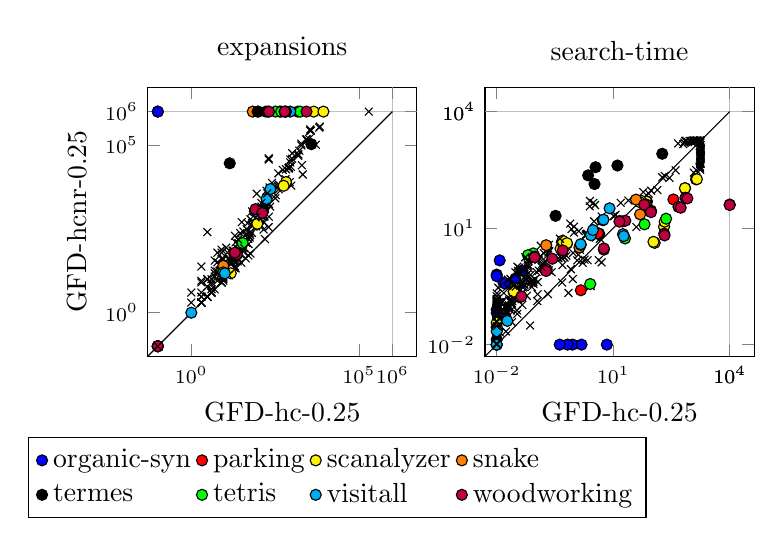
\begin{tikzpicture}
\begin{axis}[at={(0,0)}, extra x tick style={grid=major}, extra x ticks=1000000, extra y tick style={grid=major}, extra y ticks=1000000, height=5cm, legend cell align=left, legend style={at={(1.0, -0.5)}}, title=expansions, width=5cm, xlabel=GFD-hc-0.25, xmin=0.05, xmode=log, ylabel=GFD-hcnr-0.25, ymin=0.05, ymode=log]

\addplot[color=black, mark=x, mark options={{draw=black}}, only marks, forget plot] coordinates {
(202, 357) (0.100000, 0.100000) (157, 157) (42, 42)
};
%\addlegendentry{airport}
\addplot[color=cyan, mark=x, mark options={{draw=black}}, only marks, forget plot] coordinates {
(23, 84) (34, 84)
};
%\addlegendentry{barman}
\addplot[color=magenta, mark=x, mark options={{draw=black}}, only marks, forget plot] coordinates {
(216, 5449) (139, 1000000) (0.100000, 0.100000) (158, 1230) (3, 3) (36, 264) (18, 56) (3, 10) (32, 504) (17, 62) (6, 32) (1, 1) (40, 136) (12, 62) (19, 22) (2, 2) (6, 17) (473, 1000000) (65, 1056) (9, 12)
};
%\addlegendentry{blocks}
\addplot[color=red, mark=x, mark options={{draw=black}}, only marks, forget plot] coordinates {
(35, 88) (0.100000, 0.100000) (15, 35) (11, 87) (41, 203) (13, 42)
};
%\addlegendentry{depot}
\addplot[color=yellow, mark=x, mark options={{draw=black}}, only marks, forget plot] coordinates {
(4, 10) (0.100000, 0.100000) (206, 1701) (20, 24) (51, 112) (65, 475) (255, 7472) (26, 40) (8, 8) (20, 198) (143, 304) (78, 480)
};
%\addlegendentry{driverlog}
\addplot[color=cyan, mark=x, mark options={{draw=black}}, only marks, forget plot] coordinates {
(0.100000, 0.100000)
};
%\addlegendentry{freecell}
\addplot[color=magenta, mark=x, mark options={{draw=black}}, only marks, forget plot] coordinates {
(0.100000, 0.100000)
};
%\addlegendentry{grid}
\addplot[color=black, mark=x, mark options={{draw=black}}, only marks, forget plot] coordinates {
(45, 308) (208, 1776) (668, 19057) (0.100000, 0.100000) (1920, 97200)
};
%\addlegendentry{gripper}
\addplot[color=green, mark=x, mark options={{draw=black}}, only marks, forget plot] coordinates {
(0.100000, 0.100000) (4, 4) (8, 8)
};
%\addlegendentry{hiking}
\addplot[color=red, mark=x, mark options={{draw=black}}, only marks, forget plot] coordinates {
(91, 591) (64, 241) (25, 116) (2, 24) (15, 36) (1027, 57316) (818, 20864) (156, 1310) (405, 4822) (15, 30) (9, 11) (1671, 68464) (1, 1) (0.100000, 0.100000) (26, 116) (9, 20) (535, 18210) (320, 2596) (226, 1464) (36, 129) (133, 740) (14, 16) (175, 4388) (19, 52)
};
%\addlegendentry{logistics}
\addplot[color=black, mark=x, mark options={{draw=black}}, only marks, forget plot] coordinates {
(819, 21330) (14, 37) (18, 37) (57, 211) (395, 5949) (1545, 47759) (166, 1634) (156, 1401) (3709, 271472) (416, 6433) (1019, 39297) (67, 396) (1542, 53181) (164, 1672) (2684, 147165) (330, 3216) (18, 71) (135, 880) (931, 22717) (6534, 333019) (4451, 1000000) (3510, 268001) (409, 6563) (1, 1) (3558, 293838) (824, 21385) (1563, 52503) (649, 9632) (0.100000, 0.100000) (55, 176) (155, 1555) (122, 747) (1908, 110504) (65, 395) (801, 20737) (2841, 136348) (907, 36976) (803, 20047) (17, 70) (67, 387) (391, 5786) (14, 36) (2768, 149220) (6865, 357205) (3249, 153494) (2, 3) (54, 190)
};
%\addlegendentry{miconic}
\addplot[color=cyan, mark=x, mark options={{draw=black}}, only marks, forget plot] coordinates {
(0.100000, 0.100000)
};
%\addlegendentry{movie}
\addplot[color=yellow, mark=x, mark options={{draw=black}}, only marks, forget plot] coordinates {
(0.100000, 0.100000)
};
%\addlegendentry{mprime}
\addplot[color=blue, mark=x, mark options={{draw=black}}, only marks, forget plot] coordinates {
(0.100000, 0.100000)
};
%\addlegendentry{mystery}
\addplot[color=red, mark=x, mark options={{draw=black}}, only marks, forget plot] coordinates {
(7, 18) (0.100000, 0.100000) (1, 1) (58, 617)
};
%\addlegendentry{nomystery}
\addplot[color=red, mark=x, mark options={{draw=black}}, only marks, forget plot] coordinates {
(204, 37149) (8, 62) (204, 40510) (6, 62)
};
%\addlegendentry{openstacks}
\addplot[color=blue, mark=*, mark options={{draw=black}}, only marks, forget plot] coordinates {
(0.100000, 0.100000) (0.100000, 1000000)
};
%\addlegendentry{organic-synthesis}
\addplot[color=blue, mark=*, mark options={{draw=black}}, only marks, forget plot] coordinates {
(0.100000, 0.100000) (0.100000, 1000000)
};
%\addlegendentry{organic-synthesis-split}
\addplot[color=blue, mark=x, mark options={{draw=black}}, only marks, forget plot] coordinates {
(21, 126) (0.100000, 0.100000)
};
%\addlegendentry{pathways-noneg}
\addplot[color=yellow, mark=x, mark options={{draw=black}}, only marks, forget plot] coordinates {
(6, 9) (0.100000, 0.100000) (3, 3) (9, 21) (2, 2) (9, 9) (9, 10) (11, 21) (25, 40) (1, 1)
};
%\addlegendentry{pipesworld-nt}
\addplot[color=green, mark=x, mark options={{draw=black}}, only marks, forget plot] coordinates {
(2, 8) (0.100000, 0.100000) (3, 3) (5, 5) (1, 1)
};
%\addlegendentry{pipesworld-t}
\addplot[color=green, mark=x, mark options={{draw=black}}, only marks, forget plot] coordinates {
(863, 7878) (29, 56) (4, 8) (2109, 13290) (55, 244) (8, 40) (9, 18) (173, 2644) (5183, 102720) (1, 2) (5, 36) (3, 3) (2, 9) (8, 76) (3, 10) (16, 29) (5, 12) (3, 6) (2, 2) (7, 28) (206, 727) (0.100000, 0.100000) (902, 30464) (25, 76) (29, 236) (5, 15) (2, 3) (116, 371) (19, 42) (151, 749) (50, 161) (9, 39) (31, 156) (149, 498) (85, 375) (196523, 1000000) (2, 4) (151, 741) (958, 6186) (9, 40)
};
%\addlegendentry{psr-small}
\addplot[color=black, mark=x, mark options={{draw=black}}, only marks, forget plot] coordinates {
(112, 430) (43, 122) (0.100000, 0.100000) (9, 12) (1997, 25113)
};
%\addlegendentry{rovers}
\addplot[color=blue, mark=x, mark options={{draw=black}}, only marks, forget plot] coordinates {
(0.100000, 0.100000) (1, 1) (89, 3559) (3, 255) (2, 2) (48, 466)
};
%\addlegendentry{satellite}
\addplot[color=yellow, mark=*, mark options={{draw=black}}, only marks, forget plot] coordinates {
(668, 7908) (4471, 1000000) (93, 448) (568, 6122) (0.100000, 0.100000) (8748, 1000000) (15, 15)
};
%\addlegendentry{scanalyzer}
\addplot[color=orange, mark=*, mark options={{draw=black}}, only marks, forget plot] coordinates {
(436, 1000000) (9, 25) (68, 1000000) (168, 1000000)
};
%\addlegendentry{snake}
\addplot[color=magenta, mark=x, mark options={{draw=black}}, only marks, forget plot] coordinates {
(0.100000, 0.100000) (24, 34) (35, 67)
};
%\addlegendentry{storage}
\addplot[color=black, mark=*, mark options={{draw=black}}, only marks, forget plot] coordinates {
(95, 1000000) (99, 1000000) (14, 28672) (193, 1000000) (3812, 106752) (1504, 1000000)
};
%\addlegendentry{termes}
\addplot[color=green, mark=*, mark options={{draw=black}}, only marks, forget plot] coordinates {
(34, 120) (325, 1000000) (480, 1000000) (9, 16) (1776, 1000000)
};
%\addlegendentry{tetris}
\addplot[color=green, mark=x, mark options={{draw=black}}, only marks, forget plot] coordinates {
(4, 7) (7, 13) (3, 3) (4, 4) (0.100000, 0.100000) (1, 1)
};
%\addlegendentry{tidybot}
\addplot[color=red, mark=x, mark options={{draw=black}}, only marks, forget plot] coordinates {
(25, 154) (0.100000, 0.100000) (123, 1478)
};
%\addlegendentry{tpp}
\addplot[color=red, mark=x, mark options={{draw=black}}, only marks, forget plot] coordinates {
(0.100000, 0.100000) (13, 13) (58, 58) (4, 5) (5, 18) (38, 84) (50, 51) (25, 40) (31, 31) (21, 21)
};
%\addlegendentry{transport}
\addplot[color=blue, mark=x, mark options={{draw=black}}, only marks, forget plot] coordinates {
(0.100000, 0.100000)
};
%\addlegendentry{trucks}
\addplot[color=cyan, mark=*, mark options={{draw=black}}, only marks, forget plot] coordinates {
(893, 1000000) (0.100000, 0.100000) (229, 4901) (670, 1000000) (79, 1059) (10, 15) (176, 2486) (1, 1)
};
%\addlegendentry{visitall}
\addplot[color=purple, mark=*, mark options={{draw=black}}, only marks, forget plot] coordinates {
(82, 1229) (0.100000, 0.100000) (131, 940) (23, 55) (617, 1000000) (208, 1000000) (2738, 1000000) (20, 62) (608, 1000000)
};
%\addlegendentry{woodworking}
\addplot[color=blue, mark=x, mark options={{draw=black}}, only marks, forget plot] coordinates {
(0.100000, 0.100000) (123, 1874) (4, 4) (394, 14323) (1, 4) (8, 8) (83, 697) (184, 3618)
};
%\addlegendentry{zenotravel}
\addplot[color=black] coordinates {(0.050000, 0.050000) (1000000, 1000000)};
\end{axis}





%search time
\begin{axis}[at={(20,0)}, extra x tick style={grid=major}, extra x ticks=10000, extra y tick style={grid=major}, extra y ticks=10000, height=5cm, legend cell align=left, legend style={at={(0.6, -0.3)}}, title=search-time, width=5cm, xlabel=GFD-hc-0.25, xmin=0.005, xmode=log, ymin=0.005, ymode=log, legend columns=4]

\addplot[color=green, mark=x, mark options={{draw=black}}, only marks, forget plot] coordinates {
(0.112780, 0.198327) (0.010000, 0.019164) (0.010000, 0.018347) (0.010000, 0.010000) (0.811526, 0.878469) (0.010000, 0.017541) (1.392966, 2.744087) (0.018178, 0.064894) (0.492103, 1.114480) (1.187180, 1.480010) (0.010000, 0.038277) (0.010000, 0.129951) (4.580029, 5.330525) (0.010000, 0.091064) (1691.842493, 1322.792929) (0.010000, 0.048113) (0.010000, 0.131445)
};
%\addlegendentry{airport}
\addplot[color=yellow, mark=x, mark options={{draw=black}}, only marks, forget plot] coordinates {
(0.033120, 0.076361) (0.018508, 0.067104) (0.018524, 0.071270) (0.017666, 0.064389)
};
%\addlegendentry{barman}
\addplot[color=black, mark=x, mark options={{draw=black}}, only marks, forget plot] coordinates {
(0.106117, 0.747937) (0.139880, 1.130550) (0.023761, 0.144192) (0.022883, 0.135841) (5.020920, 19.857987) (0.051333, 0.355636) (0.011663, 0.058854) (0.010000, 0.010000) (0.056137, 0.467749) (0.049992, 0.308721) (0.210779, 2.071900) (0.010000, 0.022584) (0.214123, 2.347050) (0.010000, 0.021646) (0.011186, 0.052181) (0.225803, 2.580250) (0.010000, 0.024214) (0.014036, 0.073485) (1.267270, 2.061785) (0.023624, 0.120193)
};
%\addlegendentry{blocks}
\addplot[color=green, mark=x, mark options={{draw=black}}, only marks, forget plot] coordinates {
(0.047089, 0.296653) (0.010074, 0.063875) (0.020327, 0.088525) (0.051365, 0.349580) (0.012141, 0.123813) (0.010000, 0.010000)
};
%\addlegendentry{depot}
\addplot[color=red, mark=x, mark options={{draw=black}}, only marks, forget plot] coordinates {
(0.054591, 0.512738) (0.011820, 0.030213) (0.087964, 0.362773) (0.044791, 0.215811) (0.222812, 3.707570) (0.027948, 0.219084) (0.096936, 0.482844) (0.012750, 0.072234) (0.080414, 0.303832) (0.237527, 1.795440) (0.010000, 0.010000) (0.023106, 0.076168) (0.010000, 0.013002)
};
%\addlegendentry{driverlog}
\addplot[color=blue, mark=x, mark options={{draw=black}}, only marks, forget plot] coordinates {
(1.826977, 1.545542) (0.110795, 0.131787) (0.208937, 0.199343) (0.010000, 0.029874) (2.632227, 0.323642) (0.072462, 0.031164) (4.240369, 1.496790) (0.912273, 0.487512) (1.645699, 1.275004) (0.703899, 0.213877) (0.485120, 0.397746) (5.025293, 1.308984) (2.182068, 1.488412)
};
%\addlegendentry{floortile}
\addplot[color=yellow, mark=x, mark options={{draw=black}}, only marks, forget plot] coordinates {
(0.010000, 0.096289) (0.010000, 0.014482) (0.010000, 0.123179) (0.010000, 0.135099) (0.010000, 0.139748) (0.010000, 0.149630) (0.010000, 0.103611) (0.010000, 0.084542) (0.010000, 0.084437) (0.010000, 0.054917) (0.010000, 0.068708) (0.010000, 0.030907) (0.010000, 0.095698) (0.010000, 0.130291) (0.010000, 0.072304)
};
%\addlegendentry{freecell}
\addplot[color=black, mark=x, mark options={{draw=black}}, only marks, forget plot] coordinates {
(0.010000, 0.045548) (0.010000, 0.010000)
};
%\addlegendentry{grid}
\addplot[color=green, mark=x, mark options={{draw=black}}, only marks, forget plot] coordinates {
(3.613340, 5.745380) (0.114229, 0.410417) (69.428800, 40.124500) (1683.969572, 374.027407) (1731.840130, 675.209617) (0.010000, 0.010000) (0.010002, 0.043612)
};
%\addlegendentry{gripper}
\addplot[color=green, mark=x, mark options={{draw=black}}, only marks, forget plot] coordinates {
(0.010000, 0.010240) (0.017259, 0.021861) (0.010000, 0.010000)
};
%\addlegendentry{hiking}
\addplot[color=red, mark=x, mark options={{draw=black}}, only marks, forget plot] coordinates {
(0.010000, 0.015940) (0.842363, 9.437350) (2.520830, 49.982100) (0.087762, 0.401981) (0.010000, 0.030010) (0.024731, 0.115098) (2.491980, 36.400500) (0.010000, 0.010000) (0.036979, 0.278576) (0.975676, 10.958800) (0.010000, 0.016523) (0.042243, 0.369600) (0.088012, 0.453266) (0.010000, 0.029815) (0.119733, 1.526640) (0.010000, 0.018769) (0.218992, 0.812916) (0.389319, 1.670570) (0.056266, 0.609610)
};
%\addlegendentry{logistics}
\addplot[color=red, mark=x, mark options={{draw=black}}, only marks, forget plot] coordinates {
(1758.454883, 451.723072) (1784.555846, 625.046578) (1783.392960, 612.141613) (1739.302574, 315.409800) (1396.936730, 1790.859860) (0.020543, 0.102587) (1343.458600, 1780.345654) (1214.667700, 1785.381126) (1774.367246, 832.812426) (1236.519400, 1790.911845) (1695.170330, 1755.414627) (1457.695990, 1784.833575) (95.121600, 92.007100) (1773.630863, 714.656261) (0.010000, 0.024856) (0.080417, 0.431161) (1797.424218, 1073.010056) (0.019771, 0.087963) (1742.421455, 516.392804) (3.643930, 7.914840) (1766.092324, 684.277191) (0.010000, 0.010000) (0.556232, 1.753830) (59.216700, 84.367300) (1770.699554, 813.426270) (280.593000, 196.950000) (1762.724350, 1787.997528) (0.043562, 0.203888) (1776.515704, 933.195019) (0.010000, 0.010201) (0.010905, 0.039571) (0.024835, 0.105955) (0.462530, 1.714130) (2.002460, 6.883860) (0.624117, 1.953380) (24.527300, 51.269600) (137.616000, 95.702500) (1124.430200, 1771.940824) (1755.182973, 480.461774) (0.924303, 2.292340) (0.035658, 0.144173) (1777.739008, 1103.700284) (1754.296950, 620.511863) (4.916260, 14.665700) (2.071620, 6.913400) (1701.857381, 351.829898) (1664.944000, 1790.999986) (1775.961989, 917.895716) (82.159600, 77.440900) (1794.476710, 924.925172) (932.102000, 1765.103581) (0.258800, 0.731319) (1699.198990, 1794.052392) (1715.118656, 376.513908) (1188.980000, 267.526000) (213.320000, 220.455000) (718.532000, 1757.711340) (1.960510, 6.443440) (468.933000, 1516.887500) (183.425000, 203.693000) (1019.232360, 1743.105223) (0.082211, 0.432722) (1081.028100, 1595.900487) (1422.482990, 1784.569563) (1695.700665, 388.895828) (1760.736575, 733.573369) (1500.752010, 1793.952733) (1769.068892, 1372.748427) (1756.331027, 588.459928) (1756.100431, 448.431720) (1719.953112, 1632.852946) (1194.710920, 1781.446228) (0.075792, 0.392522) (676.705200, 1594.288800) (752.554100, 1772.233910) (10.288000, 20.457500) (1770.825585, 745.939521) (841.482000, 1646.701430) (2.151310, 7.150320) (1749.611400, 1794.006577) (1755.994730, 1381.614395) (0.010000, 0.023664) (1310.406500, 1754.296822) (405.371000, 308.579608) (3.208340, 14.979600) (636.977000, 1451.813900) (1379.830000, 311.706000) (1740.428873, 1671.795711) (0.010853, 0.037363) (1705.725876, 350.332301) (1769.663575, 785.902173) (1794.507620, 1043.371432) (0.083866, 0.434201) (1207.112010, 1783.736598) (0.010686, 0.037065) (0.515280, 1.878000) (1737.569132, 1532.739509) (1379.558400, 1767.764765) (10.637500, 20.334200) (11.487900, 22.044000) (1761.070289, 1141.787992)
};
%\addlegendentry{miconic}

\addplot[color=black, mark=x, mark options={{draw=black}}, only marks, forget plot] coordinates {
(0.010000, 0.050826) (0.010000, 0.035596) (0.010000, 0.016542) (0.010000, 0.020320) (0.010000, 0.011074) (0.010000, 0.021827) (0.010000, 0.028115) (0.010000, 0.010000) (0.010000, 0.010863) (0.010000, 0.019874) (0.010000, 0.012505)
};
%\addlegendentry{mprime}
\addplot[color=magenta, mark=x, mark options={{draw=black}}, only marks, forget plot] coordinates {
(0.010000, 0.042143) (0.010000, 0.086483) (0.010000, 0.041073) (0.010000, 0.016675) (0.010000, 0.052047) (0.010000, 0.010000) (0.010000, 0.026462) (0.010000, 0.017516) (0.010000, 0.013411)
};
%\addlegendentry{mystery}
\addplot[color=blue, mark=x, mark options={{draw=black}}, only marks, forget plot] coordinates {
(0.033859, 0.061799) (0.010000, 0.011833) (0.010000, 0.020266) (0.010000, 0.016874) (0.164108, 2.244940) (0.010000, 0.029445) (0.011152, 0.125176) (0.010000, 0.010000) (0.024699, 0.037792) (0.133764, 1.914530) (0.010000, 0.080387)
};
%\addlegendentry{nomystery}
\addplot[color=blue, mark=x, mark options={{draw=black}}, only marks, forget plot] coordinates {
(0.010000, 0.020682) (0.010000, 0.023188) (0.010000, 0.021022) (0.010000, 0.020747) (3.087890, 45.054300) (0.010000, 0.022248) (3.391240, 39.355500)
};
%\addlegendentry{openstacks}


\addplot[color=blue, mark=*, mark options={{draw=black}}, only marks] coordinates {
(0.010000, 0.079843) (0.011918, 1.476270) (0.010000, 0.065329) (0.898165, 0.010000) (0.010000, 0.635602) (0.010000, 0.010000) (0.010000, 0.578103)
};
\addlegendentry{organic-syn}

\addplot[color=blue, mark=*, mark options={{draw=black}}, only marks, forget plot] coordinates {
(1.529610, 0.010000) (6.852800, 0.010000) (0.665566, 0.010000) (0.015000, 0.387728) (0.030260, 0.501791) (0.046129, 0.799463) (0.010000, 0.013611) (0.418922, 0.010000) (0.080380, 1.797640) (0.016974, 0.375984)
};
%\addlegendentry{organic-synthesis-split}

\addplot[color=red, mark=*, mark options={{draw=black}}, only marks] coordinates {
(354.308000, 54.747826) (4.369680, 7.156315) (4.158310, 7.071952) (1.467470, 0.250811) (4.034000, 7.362436)
};
\addlegendentry{parking}



\addplot[color=magenta, mark=x, mark options={{draw=black}}, only marks, forget plot] coordinates {
(0.025173, 0.131342) (0.010000, 0.010000)
};
%\addlegendentry{pathways-noneg}
\addplot[color=red, mark=x, mark options={{draw=black}}, only marks, forget plot] coordinates {
(0.010029, 0.060251) (0.015292, 0.212873) (0.010000, 0.022947) (0.011442, 0.087135) (0.010000, 0.018068) (0.010000, 0.031865) (0.010000, 0.020019) (0.010000, 0.010141) (0.010000, 0.011517) (0.058710, 0.616928) (0.010000, 0.040296) (0.010000, 0.010000) (0.010000, 0.077459) (0.013224, 0.116769) (0.016760, 0.055870) (0.010000, 0.112948)
};
%\addlegendentry{pipesworld-nt}
\addplot[color=cyan, mark=x, mark options={{draw=black}}, only marks, forget plot] coordinates {
(0.010000, 0.054725) (0.010000, 0.121619) (0.018624, 0.309852) (0.010000, 0.208573) (0.010000, 0.013535) (0.010000, 0.031144) (0.010000, 0.010000) (0.010000, 0.027756) (0.010000, 0.082473) (0.010000, 0.105976) (0.037226, 0.948894)
};
%\addlegendentry{pipesworld-t}
\addplot[color=cyan, mark=x, mark options={{draw=black}}, only marks, forget plot] coordinates {
(0.167634, 1.259400) (0.016539, 0.090135) (0.010000, 0.025280) (0.076559, 0.428527) (0.016052, 0.051106) (0.013182, 0.049950) (0.010000, 0.010204) (0.020196, 0.092624) (0.782098, 13.053100) (0.010000, 0.030015) (0.010000, 0.041169) (0.010000, 0.018507) (0.173249, 1.404480) (0.010000, 0.010665) (71.364600, 41.776722) (0.010000, 0.022326) (1.298010, 8.390570) (0.016500, 0.097702) (0.010000, 0.017507) (0.010993, 0.042908) (0.121458, 0.800345) (0.059695, 0.180480) (0.010000, 0.010294) (0.010000, 0.010000)
};
%\addlegendentry{psr-small}
\addplot[color=red, mark=x, mark options={{draw=black}}, only marks, forget plot] coordinates {
(0.045690, 0.105527) (0.020222, 0.055336) (0.010000, 0.025106) (39.464200, 10.708100) (0.010000, 0.010000)
};
%\addlegendentry{rovers}
\addplot[color=blue, mark=x, mark options={{draw=black}}, only marks, forget plot] coordinates {
(0.020869, 0.137167) (0.031974, 0.282129) (0.135445, 3.531220) (0.021938, 0.092936) (0.010000, 0.010000)
};
%\addlegendentry{satellite}
\addplot[color=yellow, mark=*, mark options={{draw=black}}, only marks] coordinates {
(203.426453, 10.813615) (74.017800, 48.652022) (211.909232, 14.681458) (0.028347, 0.222258) (116.788644, 4.171740) (1355.398989, 180.049969) (0.027595, 0.227983) (0.643558, 3.985290) (71.621600, 48.346642) (0.027768, 0.217251) (708.724017, 106.487008) (51.352900, 51.223346) (108.806030, 4.432177) (0.440953, 2.915580) (47.885800, 46.914166) (0.027464, 0.232904) (0.479151, 4.401790) (0.010000, 0.028035) (703.002174, 106.674992) (1427.805137, 181.877305) (0.495834, 4.737220) (0.645675, 4.098930) (0.010000, 0.036820)
};
\addlegendentry{scanalyzer}
\addplot[color=orange, mark=*, mark options={{draw=black}}, only marks] coordinates {
(38.648530, 54.249486) (49.235100, 22.591818) (0.187869, 3.629110) (0.010000, 0.010000) (1.347050, 3.183905) (1.458500, 3.711125)
};
\addlegendentry{snake}
\addplot[color=yellow, mark=x, mark options={{draw=black}}, only marks, forget plot] coordinates {
(0.010000, 0.023979) (0.010000, 0.023523) (0.019200, 0.095873) (0.011441, 0.030044) (0.010000, 0.010000) (0.010000, 0.040493)
};
%\addlegendentry{storage}
\addplot[color=black, mark=*, mark options={{draw=black}}, only marks] coordinates {
(0.327863, 20.734600) (183.306000, 821.597441) (3.508920, 369.800274) (3.310920, 136.234000) (2.260760, 228.032686) (12.841000, 409.058131)
};
\addlegendentry{termes}
\addplot[color=green, mark=*, mark options={{draw=black}}, only marks] coordinates {
(0.087094, 2.231570) (2.559430, 0.363580) (20.143500, 5.420359) (0.063869, 2.008870) (63.796000, 12.543131) (230.241303, 17.483130)
};
\addlegendentry{tetris}
\addplot[color=blue, mark=x, mark options={{draw=black}}, only marks, forget plot] coordinates {
(0.019319, 0.473506) (0.042040, 0.648883) (0.027109, 0.323255) (0.037462, 0.723225) (0.035466, 0.786945) (0.065097, 1.070840) (0.030351, 0.729299) (0.080278, 1.611100) (0.022600, 0.489540) (0.054421, 1.780740) (0.066010, 0.931967) (0.033915, 1.014210) (0.065018, 1.382880) (0.038939, 0.726956) (0.026864, 0.358107) (0.050462, 0.854148) (0.073953, 0.623370) (0.010000, 0.175639) (0.042476, 0.448563) (0.103977, 1.592870) (0.010952, 0.290943) (0.062857, 1.160410) (0.062862, 1.537910)
};
%\addlegendentry{tidybot}
\addplot[color=blue, mark=x, mark options={{draw=black}}, only marks, forget plot] coordinates {
(0.010000, 0.010000) (0.010000, 0.052804) (0.046523, 0.369383)
};
%\addlegendentry{tpp}
\addplot[color=green, mark=x, mark options={{draw=black}}, only marks, forget plot] coordinates {
(0.010000, 0.023169) (0.010000, 0.064205) (0.029663, 0.147973) (0.010000, 0.038112) (0.010000, 0.010672) (0.010000, 0.010000) (0.010000, 0.039217) (0.012020, 0.020608) (0.010000, 0.059111) (0.010000, 0.021860) (0.010000, 0.057709) (0.010000, 0.017416) (0.010000, 0.011923) (0.010000, 0.014073) (0.010000, 0.028013) (0.010000, 0.012332)
};
%\addlegendentry{transport}
\addplot[color=magenta, mark=x, mark options={{draw=black}}, only marks, forget plot] coordinates {
(0.010000, 0.010000)
};
%\addlegendentry{trucks}
\addplot[color=cyan, mark=*, mark options={{draw=black}}, only marks] coordinates {
(17.853300, 6.986764) (5.372019, 15.997092) (1.451020, 3.850950) (2.658960, 6.552700) (8.048821, 32.363919) (5.617487, 16.460272) (3.008980, 8.905630) (0.010000, 0.010000) (0.010000, 0.021872) (0.018731, 0.040848) (18.687500, 6.229438)
};
\addlegendentry{visitall}
\addplot[color=purple, mark=*, mark options={{draw=black}}, only marks] coordinates {
(205.160000, 7.237639) (723.500819, 60.597384) (0.270261, 1.627080) (478.960000, 35.206969) (71.184424, 40.509067) (14.716000, 15.257454) (17.274288, 14.872363) (10000, 40.471993) (5.732910, 2.777757) (0.095040, 1.835804) (812.101823, 58.104613) (0.193118, 0.870327) (0.185642, 0.785668) (20.525555, 15.476348) (0.043164, 0.173316) (210.175000, 6.488662) (0.094698, 1.770294) (93.950510, 28.189315) (5.738660, 3.002524) (62.870901, 39.979857) (94.167276, 25.744202) (546.009000, 33.469259) (0.502560, 2.670380) (14.487000, 14.666541) (10000, 39.328732)
};
\addlegendentry{woodworking}
\addplot[color=cyan, mark=x, mark options={{draw=black}}, only marks, forget plot] coordinates {
(15.639000, 44.734700) (0.010000, 0.014936) (0.426344, 5.324050) (0.978021, 7.639780) (0.010000, 0.029947) (0.010000, 0.010488) (0.030934, 0.310911) (0.010000, 0.010000) (0.014032, 0.132001) (0.010000, 0.010557) (0.141588, 1.013860)
};
%\addlegendentry{zenotravel}
\addplot[color=black] coordinates {(0.0050000, 0.0050000) (10000, 10000)};
\end{axis}
\end{tikzpicture}
	\end{minipage}
	%\hfill
	%\begin{minipage}{0.2\textwidth}
	%	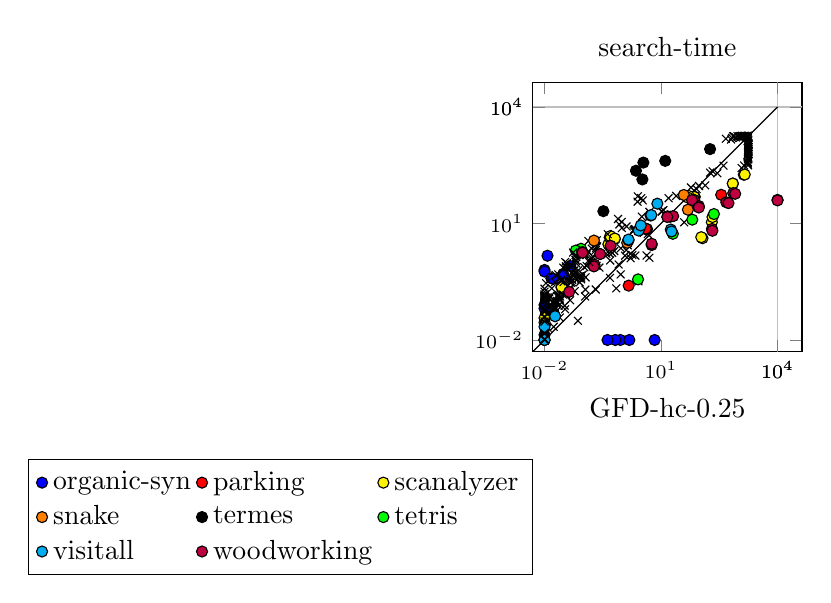
\begin{tikzpicture}
\begin{axis}[extra x tick style={grid=major}, extra x ticks=10000, extra y tick style={grid=major}, extra y ticks=10000, height=5cm, legend cell align=left, legend style={at={(0.0, -0.4)}}, title=search-time, width=5cm, xlabel=GFD-hc-0.25, xmin=0.005, xmode=log, ymin=0.005, ymode=log, legend columns=3]

\addplot[color=green, mark=x, mark options={{draw=black}}, only marks, forget plot] coordinates {
(0.112780, 0.198327) (0.010000, 0.019164) (0.010000, 0.018347) (0.010000, 0.010000) (0.811526, 0.878469) (0.010000, 0.017541) (1.392966, 2.744087) (0.018178, 0.064894) (0.492103, 1.114480) (1.187180, 1.480010) (0.010000, 0.038277) (0.010000, 0.129951) (4.580029, 5.330525) (0.010000, 0.091064) (1691.842493, 1322.792929) (0.010000, 0.048113) (0.010000, 0.131445)
};
%\addlegendentry{airport}
\addplot[color=yellow, mark=x, mark options={{draw=black}}, only marks, forget plot] coordinates {
(0.033120, 0.076361) (0.018508, 0.067104) (0.018524, 0.071270) (0.017666, 0.064389)
};
%\addlegendentry{barman}
\addplot[color=black, mark=x, mark options={{draw=black}}, only marks, forget plot] coordinates {
(0.106117, 0.747937) (0.139880, 1.130550) (0.023761, 0.144192) (0.022883, 0.135841) (5.020920, 19.857987) (0.051333, 0.355636) (0.011663, 0.058854) (0.010000, 0.010000) (0.056137, 0.467749) (0.049992, 0.308721) (0.210779, 2.071900) (0.010000, 0.022584) (0.214123, 2.347050) (0.010000, 0.021646) (0.011186, 0.052181) (0.225803, 2.580250) (0.010000, 0.024214) (0.014036, 0.073485) (1.267270, 2.061785) (0.023624, 0.120193)
};
%\addlegendentry{blocks}
\addplot[color=green, mark=x, mark options={{draw=black}}, only marks, forget plot] coordinates {
(0.047089, 0.296653) (0.010074, 0.063875) (0.020327, 0.088525) (0.051365, 0.349580) (0.012141, 0.123813) (0.010000, 0.010000)
};
%\addlegendentry{depot}
\addplot[color=red, mark=x, mark options={{draw=black}}, only marks, forget plot] coordinates {
(0.054591, 0.512738) (0.011820, 0.030213) (0.087964, 0.362773) (0.044791, 0.215811) (0.222812, 3.707570) (0.027948, 0.219084) (0.096936, 0.482844) (0.012750, 0.072234) (0.080414, 0.303832) (0.237527, 1.795440) (0.010000, 0.010000) (0.023106, 0.076168) (0.010000, 0.013002)
};
%\addlegendentry{driverlog}
\addplot[color=blue, mark=x, mark options={{draw=black}}, only marks, forget plot] coordinates {
(1.826977, 1.545542) (0.110795, 0.131787) (0.208937, 0.199343) (0.010000, 0.029874) (2.632227, 0.323642) (0.072462, 0.031164) (4.240369, 1.496790) (0.912273, 0.487512) (1.645699, 1.275004) (0.703899, 0.213877) (0.485120, 0.397746) (5.025293, 1.308984) (2.182068, 1.488412)
};
%\addlegendentry{floortile}
\addplot[color=yellow, mark=x, mark options={{draw=black}}, only marks, forget plot] coordinates {
(0.010000, 0.096289) (0.010000, 0.014482) (0.010000, 0.123179) (0.010000, 0.135099) (0.010000, 0.139748) (0.010000, 0.149630) (0.010000, 0.103611) (0.010000, 0.084542) (0.010000, 0.084437) (0.010000, 0.054917) (0.010000, 0.068708) (0.010000, 0.030907) (0.010000, 0.095698) (0.010000, 0.130291) (0.010000, 0.072304)
};
%\addlegendentry{freecell}
\addplot[color=black, mark=x, mark options={{draw=black}}, only marks, forget plot] coordinates {
(0.010000, 0.045548) (0.010000, 0.010000)
};
%\addlegendentry{grid}
\addplot[color=green, mark=x, mark options={{draw=black}}, only marks, forget plot] coordinates {
(3.613340, 5.745380) (0.114229, 0.410417) (69.428800, 40.124500) (1683.969572, 374.027407) (1731.840130, 675.209617) (0.010000, 0.010000) (0.010002, 0.043612)
};
%\addlegendentry{gripper}
\addplot[color=green, mark=x, mark options={{draw=black}}, only marks, forget plot] coordinates {
(0.010000, 0.010240) (0.017259, 0.021861) (0.010000, 0.010000)
};
%\addlegendentry{hiking}
\addplot[color=red, mark=x, mark options={{draw=black}}, only marks, forget plot] coordinates {
(0.010000, 0.015940) (0.842363, 9.437350) (2.520830, 49.982100) (0.087762, 0.401981) (0.010000, 0.030010) (0.024731, 0.115098) (2.491980, 36.400500) (0.010000, 0.010000) (0.036979, 0.278576) (0.975676, 10.958800) (0.010000, 0.016523) (0.042243, 0.369600) (0.088012, 0.453266) (0.010000, 0.029815) (0.119733, 1.526640) (0.010000, 0.018769) (0.218992, 0.812916) (0.389319, 1.670570) (0.056266, 0.609610)
};
%\addlegendentry{logistics}
\addplot[color=red, mark=x, mark options={{draw=black}}, only marks, forget plot] coordinates {
(1758.454883, 451.723072) (1784.555846, 625.046578) (1783.392960, 612.141613) (1739.302574, 315.409800) (1396.936730, 1790.859860) (0.020543, 0.102587) (1343.458600, 1780.345654) (1214.667700, 1785.381126) (1774.367246, 832.812426) (1236.519400, 1790.911845) (1695.170330, 1755.414627) (1457.695990, 1784.833575) (95.121600, 92.007100) (1773.630863, 714.656261) (0.010000, 0.024856) (0.080417, 0.431161) (1797.424218, 1073.010056) (0.019771, 0.087963) (1742.421455, 516.392804) (3.643930, 7.914840) (1766.092324, 684.277191) (0.010000, 0.010000) (0.556232, 1.753830) (59.216700, 84.367300) (1770.699554, 813.426270) (280.593000, 196.950000) (1762.724350, 1787.997528) (0.043562, 0.203888) (1776.515704, 933.195019) (0.010000, 0.010201) (0.010905, 0.039571) (0.024835, 0.105955) (0.462530, 1.714130) (2.002460, 6.883860) (0.624117, 1.953380) (24.527300, 51.269600) (137.616000, 95.702500) (1124.430200, 1771.940824) (1755.182973, 480.461774) (0.924303, 2.292340) (0.035658, 0.144173) (1777.739008, 1103.700284) (1754.296950, 620.511863) (4.916260, 14.665700) (2.071620, 6.913400) (1701.857381, 351.829898) (1664.944000, 1790.999986) (1775.961989, 917.895716) (82.159600, 77.440900) (1794.476710, 924.925172) (932.102000, 1765.103581) (0.258800, 0.731319) (1699.198990, 1794.052392) (1715.118656, 376.513908) (1188.980000, 267.526000) (213.320000, 220.455000) (718.532000, 1757.711340) (1.960510, 6.443440) (468.933000, 1516.887500) (183.425000, 203.693000) (1019.232360, 1743.105223) (0.082211, 0.432722) (1081.028100, 1595.900487) (1422.482990, 1784.569563) (1695.700665, 388.895828) (1760.736575, 733.573369) (1500.752010, 1793.952733) (1769.068892, 1372.748427) (1756.331027, 588.459928) (1756.100431, 448.431720) (1719.953112, 1632.852946) (1194.710920, 1781.446228) (0.075792, 0.392522) (676.705200, 1594.288800) (752.554100, 1772.233910) (10.288000, 20.457500) (1770.825585, 745.939521) (841.482000, 1646.701430) (2.151310, 7.150320) (1749.611400, 1794.006577) (1755.994730, 1381.614395) (0.010000, 0.023664) (1310.406500, 1754.296822) (405.371000, 308.579608) (3.208340, 14.979600) (636.977000, 1451.813900) (1379.830000, 311.706000) (1740.428873, 1671.795711) (0.010853, 0.037363) (1705.725876, 350.332301) (1769.663575, 785.902173) (1794.507620, 1043.371432) (0.083866, 0.434201) (1207.112010, 1783.736598) (0.010686, 0.037065) (0.515280, 1.878000) (1737.569132, 1532.739509) (1379.558400, 1767.764765) (10.637500, 20.334200) (11.487900, 22.044000) (1761.070289, 1141.787992)
};
%\addlegendentry{miconic}

\addplot[color=black, mark=x, mark options={{draw=black}}, only marks, forget plot] coordinates {
(0.010000, 0.050826) (0.010000, 0.035596) (0.010000, 0.016542) (0.010000, 0.020320) (0.010000, 0.011074) (0.010000, 0.021827) (0.010000, 0.028115) (0.010000, 0.010000) (0.010000, 0.010863) (0.010000, 0.019874) (0.010000, 0.012505)
};
%\addlegendentry{mprime}
\addplot[color=magenta, mark=x, mark options={{draw=black}}, only marks, forget plot] coordinates {
(0.010000, 0.042143) (0.010000, 0.086483) (0.010000, 0.041073) (0.010000, 0.016675) (0.010000, 0.052047) (0.010000, 0.010000) (0.010000, 0.026462) (0.010000, 0.017516) (0.010000, 0.013411)
};
%\addlegendentry{mystery}
\addplot[color=blue, mark=x, mark options={{draw=black}}, only marks, forget plot] coordinates {
(0.033859, 0.061799) (0.010000, 0.011833) (0.010000, 0.020266) (0.010000, 0.016874) (0.164108, 2.244940) (0.010000, 0.029445) (0.011152, 0.125176) (0.010000, 0.010000) (0.024699, 0.037792) (0.133764, 1.914530) (0.010000, 0.080387)
};
%\addlegendentry{nomystery}
\addplot[color=blue, mark=x, mark options={{draw=black}}, only marks, forget plot] coordinates {
(0.010000, 0.020682) (0.010000, 0.023188) (0.010000, 0.021022) (0.010000, 0.020747) (3.087890, 45.054300) (0.010000, 0.022248) (3.391240, 39.355500)
};
%\addlegendentry{openstacks}


\addplot[color=blue, mark=*, mark options={{draw=black}}, only marks] coordinates {
(0.010000, 0.079843) (0.011918, 1.476270) (0.010000, 0.065329) (0.898165, 0.010000) (0.010000, 0.635602) (0.010000, 0.010000) (0.010000, 0.578103)
};
\addlegendentry{organic-syn}

\addplot[color=blue, mark=*, mark options={{draw=black}}, only marks, forget plot] coordinates {
(1.529610, 0.010000) (6.852800, 0.010000) (0.665566, 0.010000) (0.015000, 0.387728) (0.030260, 0.501791) (0.046129, 0.799463) (0.010000, 0.013611) (0.418922, 0.010000) (0.080380, 1.797640) (0.016974, 0.375984)
};
%\addlegendentry{organic-synthesis-split}

\addplot[color=red, mark=*, mark options={{draw=black}}, only marks] coordinates {
(354.308000, 54.747826) (4.369680, 7.156315) (4.158310, 7.071952) (1.467470, 0.250811) (4.034000, 7.362436)
};
\addlegendentry{parking}



\addplot[color=magenta, mark=x, mark options={{draw=black}}, only marks, forget plot] coordinates {
(0.025173, 0.131342) (0.010000, 0.010000)
};
%\addlegendentry{pathways-noneg}
\addplot[color=red, mark=x, mark options={{draw=black}}, only marks, forget plot] coordinates {
(0.010029, 0.060251) (0.015292, 0.212873) (0.010000, 0.022947) (0.011442, 0.087135) (0.010000, 0.018068) (0.010000, 0.031865) (0.010000, 0.020019) (0.010000, 0.010141) (0.010000, 0.011517) (0.058710, 0.616928) (0.010000, 0.040296) (0.010000, 0.010000) (0.010000, 0.077459) (0.013224, 0.116769) (0.016760, 0.055870) (0.010000, 0.112948)
};
%\addlegendentry{pipesworld-nt}
\addplot[color=cyan, mark=x, mark options={{draw=black}}, only marks, forget plot] coordinates {
(0.010000, 0.054725) (0.010000, 0.121619) (0.018624, 0.309852) (0.010000, 0.208573) (0.010000, 0.013535) (0.010000, 0.031144) (0.010000, 0.010000) (0.010000, 0.027756) (0.010000, 0.082473) (0.010000, 0.105976) (0.037226, 0.948894)
};
%\addlegendentry{pipesworld-t}
\addplot[color=cyan, mark=x, mark options={{draw=black}}, only marks, forget plot] coordinates {
(0.167634, 1.259400) (0.016539, 0.090135) (0.010000, 0.025280) (0.076559, 0.428527) (0.016052, 0.051106) (0.013182, 0.049950) (0.010000, 0.010204) (0.020196, 0.092624) (0.782098, 13.053100) (0.010000, 0.030015) (0.010000, 0.041169) (0.010000, 0.018507) (0.173249, 1.404480) (0.010000, 0.010665) (71.364600, 41.776722) (0.010000, 0.022326) (1.298010, 8.390570) (0.016500, 0.097702) (0.010000, 0.017507) (0.010993, 0.042908) (0.121458, 0.800345) (0.059695, 0.180480) (0.010000, 0.010294) (0.010000, 0.010000)
};
%\addlegendentry{psr-small}
\addplot[color=red, mark=x, mark options={{draw=black}}, only marks, forget plot] coordinates {
(0.045690, 0.105527) (0.020222, 0.055336) (0.010000, 0.025106) (39.464200, 10.708100) (0.010000, 0.010000)
};
%\addlegendentry{rovers}
\addplot[color=blue, mark=x, mark options={{draw=black}}, only marks, forget plot] coordinates {
(0.020869, 0.137167) (0.031974, 0.282129) (0.135445, 3.531220) (0.021938, 0.092936) (0.010000, 0.010000)
};
%\addlegendentry{satellite}
\addplot[color=yellow, mark=*, mark options={{draw=black}}, only marks] coordinates {
(203.426453, 10.813615) (74.017800, 48.652022) (211.909232, 14.681458) (0.028347, 0.222258) (116.788644, 4.171740) (1355.398989, 180.049969) (0.027595, 0.227983) (0.643558, 3.985290) (71.621600, 48.346642) (0.027768, 0.217251) (708.724017, 106.487008) (51.352900, 51.223346) (108.806030, 4.432177) (0.440953, 2.915580) (47.885800, 46.914166) (0.027464, 0.232904) (0.479151, 4.401790) (0.010000, 0.028035) (703.002174, 106.674992) (1427.805137, 181.877305) (0.495834, 4.737220) (0.645675, 4.098930) (0.010000, 0.036820)
};
\addlegendentry{scanalyzer}
\addplot[color=orange, mark=*, mark options={{draw=black}}, only marks] coordinates {
(38.648530, 54.249486) (49.235100, 22.591818) (0.187869, 3.629110) (0.010000, 0.010000) (1.347050, 3.183905) (1.458500, 3.711125)
};
\addlegendentry{snake}
\addplot[color=yellow, mark=x, mark options={{draw=black}}, only marks, forget plot] coordinates {
(0.010000, 0.023979) (0.010000, 0.023523) (0.019200, 0.095873) (0.011441, 0.030044) (0.010000, 0.010000) (0.010000, 0.040493)
};
%\addlegendentry{storage}
\addplot[color=black, mark=*, mark options={{draw=black}}, only marks] coordinates {
(0.327863, 20.734600) (183.306000, 821.597441) (3.508920, 369.800274) (3.310920, 136.234000) (2.260760, 228.032686) (12.841000, 409.058131)
};
\addlegendentry{termes}
\addplot[color=green, mark=*, mark options={{draw=black}}, only marks] coordinates {
(0.087094, 2.231570) (2.559430, 0.363580) (20.143500, 5.420359) (0.063869, 2.008870) (63.796000, 12.543131) (230.241303, 17.483130)
};
\addlegendentry{tetris}
\addplot[color=blue, mark=x, mark options={{draw=black}}, only marks, forget plot] coordinates {
(0.019319, 0.473506) (0.042040, 0.648883) (0.027109, 0.323255) (0.037462, 0.723225) (0.035466, 0.786945) (0.065097, 1.070840) (0.030351, 0.729299) (0.080278, 1.611100) (0.022600, 0.489540) (0.054421, 1.780740) (0.066010, 0.931967) (0.033915, 1.014210) (0.065018, 1.382880) (0.038939, 0.726956) (0.026864, 0.358107) (0.050462, 0.854148) (0.073953, 0.623370) (0.010000, 0.175639) (0.042476, 0.448563) (0.103977, 1.592870) (0.010952, 0.290943) (0.062857, 1.160410) (0.062862, 1.537910)
};
%\addlegendentry{tidybot}
\addplot[color=blue, mark=x, mark options={{draw=black}}, only marks, forget plot] coordinates {
(0.010000, 0.010000) (0.010000, 0.052804) (0.046523, 0.369383)
};
%\addlegendentry{tpp}
\addplot[color=green, mark=x, mark options={{draw=black}}, only marks, forget plot] coordinates {
(0.010000, 0.023169) (0.010000, 0.064205) (0.029663, 0.147973) (0.010000, 0.038112) (0.010000, 0.010672) (0.010000, 0.010000) (0.010000, 0.039217) (0.012020, 0.020608) (0.010000, 0.059111) (0.010000, 0.021860) (0.010000, 0.057709) (0.010000, 0.017416) (0.010000, 0.011923) (0.010000, 0.014073) (0.010000, 0.028013) (0.010000, 0.012332)
};
%\addlegendentry{transport}
\addplot[color=magenta, mark=x, mark options={{draw=black}}, only marks, forget plot] coordinates {
(0.010000, 0.010000)
};
%\addlegendentry{trucks}
\addplot[color=cyan, mark=*, mark options={{draw=black}}, only marks] coordinates {
(17.853300, 6.986764) (5.372019, 15.997092) (1.451020, 3.850950) (2.658960, 6.552700) (8.048821, 32.363919) (5.617487, 16.460272) (3.008980, 8.905630) (0.010000, 0.010000) (0.010000, 0.021872) (0.018731, 0.040848) (18.687500, 6.229438)
};
\addlegendentry{visitall}
\addplot[color=purple, mark=*, mark options={{draw=black}}, only marks] coordinates {
(205.160000, 7.237639) (723.500819, 60.597384) (0.270261, 1.627080) (478.960000, 35.206969) (71.184424, 40.509067) (14.716000, 15.257454) (17.274288, 14.872363) (10000, 40.471993) (5.732910, 2.777757) (0.095040, 1.835804) (812.101823, 58.104613) (0.193118, 0.870327) (0.185642, 0.785668) (20.525555, 15.476348) (0.043164, 0.173316) (210.175000, 6.488662) (0.094698, 1.770294) (93.950510, 28.189315) (5.738660, 3.002524) (62.870901, 39.979857) (94.167276, 25.744202) (546.009000, 33.469259) (0.502560, 2.670380) (14.487000, 14.666541) (10000, 39.328732)
};
\addlegendentry{woodworking}
\addplot[color=cyan, mark=x, mark options={{draw=black}}, only marks, forget plot] coordinates {
(15.639000, 44.734700) (0.010000, 0.014936) (0.426344, 5.324050) (0.978021, 7.639780) (0.010000, 0.029947) (0.010000, 0.010488) (0.030934, 0.310911) (0.010000, 0.010000) (0.014032, 0.132001) (0.010000, 0.010557) (0.141588, 1.013860)
};
%\addlegendentry{zenotravel}
\addplot[color=black] coordinates {(0.0050000, 0.0050000) (10000, 10000)};
\end{axis}
\end{tikzpicture}
	%\end{minipage}
	\begin{minipage}{0.2\textwidth}
		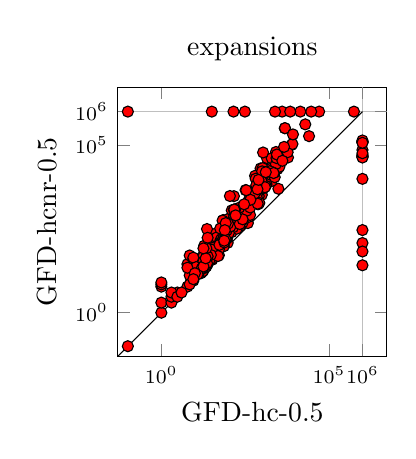
\begin{tikzpicture}
\begin{axis}[extra x tick style={grid=major}, extra x ticks=1000000, extra y tick style={grid=major}, extra y ticks=1000000, height=5cm, legend cell align=left, legend style={at={(1.3, 0.5)}}, title=expansions, width=5cm, xlabel=GFD-hc-0.5, xmin=0.05, xmode=log, ylabel=GFD-hcnr-0.5, ymin=0.05, ymode=log]
\addplot[color=red, mark=*, mark options={{draw=black}}, only marks] coordinates {
(19675, 416544) (3104, 4984) (20, 25) (63, 135) (91, 187) (121, 708) (22, 44) (13, 17) (4338, 58461) (147, 1065) (1, 6) (46, 78) (33, 65) (4955, 60566) (126, 1131) (347, 858) (95, 121) (1794, 19486) (1960, 8490) (4811, 319773) (59, 118) (15, 15) (6, 28) (29, 47) (289, 1470) (1, 1) (1000000, 125176) (70, 580) (1, 2) (32, 63) (391, 1227) (2936, 19354) (311, 1000000) (10, 13) (77, 154) (63, 223) (63, 241) (556807, 1000000) (183, 483) (56, 151) (381, 473) (649, 3465) (19, 60) (401, 720) (543, 4117) (1000000, 44409) (727, 2439) (24, 28) (195, 495) (22, 25) (1000000, 51044) (231, 928) (1069, 4857) (914, 20182) (9, 9) (97, 452) (51, 165) (354, 1334) (91, 164) (4008, 1000000) (50966, 1000000) (60, 115) (2282, 16310) (1000000, 47321) (71, 151) (28, 78) (2408, 11065) (793, 7645) (745, 2688) (16, 16) (160, 597) (55, 186) (1415, 40954) (1000000, 47120) (29498, 1000000) (8, 9) (7, 51) (17, 19) (35, 70) (60, 128) (117, 327) (449, 1726) (22, 24) (40, 227) (146, 3001) (417, 1367) (2896, 27945) (9, 40) (551, 2477) (45, 176) (1000000, 126694) (902, 6275) (17, 24) (84, 156) (43, 88) (23, 314) (2, 2) (144, 435) (179, 481) (242, 619) (987, 15235) (27, 54) (1000000, 120) (52, 52) (73, 96) (100, 316) (15, 25) (18, 18) (39, 78) (213, 931) (1000000, 122229) (12, 18) (33, 38) (1000000, 26) (17, 27) (88, 244) (2726, 58064) (2352, 15271) (2629, 62494) (137, 653) (68, 188) (17, 28) (1366, 6870) (1000000, 9853) (223, 384) (2421, 18135) (19, 100) (992, 3282) (27, 38) (5992, 42714) (1000000, 71893) (56, 99) (73, 139) (167, 592) (1960, 40507) (23, 33) (80, 153) (7560, 100166) (296, 1188) (92, 217) (17, 17) (803, 3022) (32, 1000000) (310, 867) (3331, 22681) (142, 1000000) (272, 1545) (133, 428) (158, 648) (2614, 27214) (396, 2146) (18, 48) (25480, 185128) (17, 22) (764, 1774) (11, 14) (93, 611) (151, 780) (155, 1204) (144, 689) (4881, 320447) (20, 30) (9, 44) (508, 3320) (1000000, 42693) (835, 9442) (1000000, 137745) (125, 253) (111, 3029) (59, 149) (1047, 20567) (1028, 4987) (86, 206) (1017, 5306) (443, 3510) (2159, 15261) (323, 1395) (269, 499) (352, 1385) (213, 657) (1025, 5152) (67, 561) (145, 1188) (1302, 6110) (105, 410) (443, 826) (729, 3670) (20, 22) (33, 64) (2731, 41032) (5860, 61426) (177, 319) (13, 15) (1000000, 67) (8151, 107988) (100, 410) (493, 1916) (876, 5124) (2, 3) (22, 37) (386, 1711) (67, 145) (18, 22) (259, 579) (137, 351) (103, 239) (277, 1161) (90, 288) (7, 13) (1000000, 57496) (2800, 52482) (147, 555) (625, 12152) (408, 1400) (1013, 16508) (57, 325) (92, 423) (3, 4) (2, 4) (432, 2572) (652, 9941) (78, 156) (0.100000, 1000000) (974, 8330) (82, 156) (31, 98) (6, 6) (14022, 1000000) (36, 88) (1233, 5566) (7, 7) (187, 488) (56, 100) (11, 23) (1707, 16634) (2228, 14732) (16, 21) (460, 1675) (521, 2527) (120, 438) (6986, 1000000) (32, 40) (55, 120) (8439, 208722) (12, 14) (52, 77) (723, 2514) (1000000, 292) (765, 1714) (3, 3) (18, 34) (352, 1102) (4, 4) (4084, 34055) (32, 76) (678, 6371) (19, 25) (602, 3537) (6, 22) (212, 1362) (28, 39) (23, 30) (49, 49) (115, 374) (446, 1378) (837, 1886) (0.100000, 0.100000) (737, 4825) (30, 53) (18, 24) (24, 48) (219, 442) (10, 15) (9, 10) (97, 453) (24, 172) (326, 4556) (83, 471) (792, 9194) (746, 1794) (159, 1180) (22, 84) (1084, 60319) (1, 7) (150, 1196) (57, 113) (1304, 15612) (266, 611) (454, 2342) (295, 1720) (340, 4510) (1000000, 117250) (1, 8) (21, 42) (54, 106) (76, 125) (18, 83) (2459, 1000000) (78, 290) (164, 801) (4582, 88624) (75, 141)
};
\addplot[color=black] coordinates {(0.050000, 0.050000) (1000000, 1000000)};
\end{axis}
\end{tikzpicture}
	\end{minipage}
	\hfill
	\begin{minipage}{0.2\textwidth}
		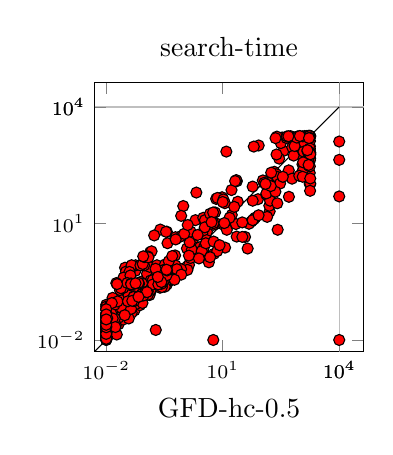
\begin{tikzpicture}
\begin{axis}[extra x tick style={grid=major}, extra x ticks=10000, extra y tick style={grid=major}, extra y ticks=10000, height=5cm, legend cell align=left, legend style={at={(1.3, 0.5)}}, title=search-time, width=5cm, xlabel=GFD-hc-0.5, xmin=0.005, xmode=log, ymin=0.005, ymode=log]
\addplot[color=red, mark=*, mark options={{draw=black}}, only marks] coordinates {
(0.141600, 0.205991) (1605.181010, 1782.630193) (12.400500, 709.237212) (1774.631742, 1791.371591) (212.897000, 213.781000) (1597.457079, 1787.500706) (0.010319, 0.015237) (0.010000, 0.013313) (863.055716, 800.358567) (161.787000, 20.520400) (0.032666, 0.692598) (0.013479, 0.026574) (0.010000, 0.080420) (0.135948, 1.828040) (0.010000, 0.028430) (1.796240, 2.829000) (1.984320, 12.173801) (3.303470, 1.674940) (0.010000, 0.043398) (0.016543, 0.053114) (0.025542, 0.044333) (0.121820, 0.184119) (0.168530, 0.410830) (0.012618, 0.020525) (0.010000, 0.033399) (0.026364, 0.060622) (4.466420, 9.015970) (0.020841, 0.025520) (0.030609, 0.725866) (1.679430, 2.531030) (0.024297, 0.112212) (68.796900, 14.125500) (1.390020, 1.946460) (1776.725506, 100.854000) (0.788609, 4.536800) (0.147242, 1.920020) (0.038869, 0.098166) (0.054435, 0.136739) (0.052649, 0.114803) (10000, 1288.588000) (0.229876, 0.280588) (213.965000, 71.343100) (0.963672, 28.123200) (0.042179, 0.050949) (1035.330000, 1076.700000) (0.010000, 0.013908) (1759.657028, 974.054000) (1.492400, 6.166240) (0.053980, 0.175691) (0.010000, 0.028648) (2.610900, 2.456000) (0.363100, 0.265775) (171.834000, 154.185000) (1748.862219, 437.770512) (0.022541, 0.192919) (1742.277675, 600.521000) (43.841020, 2.263690) (0.053471, 0.057716) (657.472000, 1639.216890) (0.010000, 0.013867) (0.010000, 0.012813) (23.112800, 122.746618) (1792.165384, 668.624000) (517.348000, 175.860757) (0.010000, 0.014193) (1141.176315, 222.928593) (2.094300, 62.526700) (0.132282, 0.297586) (364.983000, 738.802000) (0.179643, 0.248789) (0.033976, 0.177096) (0.035529, 0.075130) (0.027296, 0.033509) (1642.465839, 357.570093) (7.014660, 9.886150) (0.037661, 0.140381) (0.051290, 0.104818) (1.200340, 2.270120) (80.883000, 42.110400) (21.769200, 9.692210) (0.014665, 0.039348) (506.218000, 48.598300) (0.010000, 0.018679) (0.051869, 0.133156) (1544.759437, 662.071654) (0.842484, 0.519499) (3.924020, 6.153700) (1014.600300, 607.664400) (0.292963, 0.368375) (0.056452, 0.602398) (0.081629, 0.127455) (0.037487, 0.542903) (0.316635, 0.362635) (1745.910537, 782.198297) (0.095442, 0.154585) (0.108046, 0.181748) (143.962000, 114.253723) (0.057398, 0.837497) (0.010000, 0.015065) (1644.472263, 430.551327) (0.010000, 0.025100) (0.010000, 0.018582) (1293.739967, 1775.815607) (0.145030, 0.556515) (243.131000, 184.626000) (0.038805, 0.085258) (1573.078902, 1297.051258) (1509.464011, 319.440000) (1594.828483, 283.030432) (58.959700, 89.035000) (5.726360, 9.259810) (0.142722, 0.188514) (0.139915, 0.398103) (84.350000, 1020.977500) (0.606088, 4.426350) (0.045251, 0.050205) (0.016905, 0.051003) (0.378767, 3.103980) (0.063923, 0.118866) (0.209098, 0.550420) (10000, 434.963000) (0.010000, 0.011175) (0.010000, 0.012076) (1690.129018, 583.678216) (1132.060000, 335.230000) (0.011225, 0.048642) (0.050519, 0.127798) (1743.950000, 105.568000) (0.032207, 0.574108) (107.928000, 128.269000) (5.111340, 14.110000) (17.077100, 16.607600) (1764.370088, 1327.216581) (1744.796741, 1766.736909) (0.810539, 0.607690) (0.010000, 0.072115) (6.353300, 19.268300) (1781.313923, 474.756375) (10000, 49.701170) (131.756000, 55.826500) (0.010000, 0.010191) (0.010000, 0.011540) (24.367532, 36.344775) (1513.629800, 1776.329173) (0.028443, 0.064004) (0.010000, 0.013149) (1555.867400, 1771.592487) (1431.991213, 1633.463747) (965.037700, 1768.281767) (10.605100, 9.221870) (0.364238, 6.135960) (0.073838, 0.078722) (0.088611, 0.330700) (3.221300, 2.335110) (0.592593, 1.503610) (0.033561, 0.055405) (3.152690, 13.984400) (0.010000, 0.020071) (0.023063, 0.081845) (1583.564615, 1770.259720) (0.043392, 0.065043) (1669.949275, 1783.849378) (1292.881811, 1384.635340) (1.603190, 2.111190) (0.010000, 0.037855) (9.612490, 47.243000) (5.724610, 0.010000) (0.112374, 0.505523) (0.719389, 0.592205) (0.130703, 0.765324) (0.012547, 0.021201) (0.045001, 0.841257) (0.459686, 0.345487) (615.567009, 916.520000) (1336.381930, 356.063400) (502.109000, 233.070355) (0.118658, 1.418180) (22.377221, 130.645563) (6.775020, 42.936100) (0.161210, 0.238173) (54.475400, 11.175800) (0.281078, 0.322987) (1.410870, 3.270000) (1547.352071, 397.946658) (1671.122541, 340.823456) (0.094459, 0.832595) (253.771000, 159.234000) (139.309000, 14.788500) (0.055814, 0.082215) (1684.007832, 378.158193) (0.031498, 0.081381) (2.980340, 5.604690) (1.355710, 0.859297) (0.341617, 0.791681) (1255.796492, 1185.567220) (0.010000, 0.032813) (1577.170816, 1744.593233) (0.322172, 0.234947) (338.098300, 1630.036190) (0.010000, 0.012895) (5.763040, 10.208700) (0.202068, 0.838355) (0.344263, 0.668028) (0.018704, 0.013822) (0.039765, 0.565614) (7.298160, 45.514100) (859.125804, 1719.692730) (0.185029, 0.256387) (0.130545, 0.143080) (1.236170, 0.638606) (0.610327, 0.827987) (0.027800, 0.402353) (0.473300, 0.362876) (0.076035, 0.836031) (0.020849, 0.037541) (0.197523, 0.322307) (0.246567, 6.975030) (248.379000, 1723.736350) (11.497600, 2.390850) (0.032499, 0.046238) (10.405000, 41.573500) (1745.802918, 855.196555) (1772.045589, 1797.929785) (0.105201, 0.268812) (1739.900000, 200.420000) (0.014566, 0.121553) (1.478300, 1.292686) (0.038131, 0.035790) (0.037098, 0.070983) (0.087283, 0.907104) (0.134314, 0.195161) (0.189876, 0.442255) (15.001300, 13.975400) (313.664000, 1173.763400) (1792.403507, 106.331000) (0.208702, 0.248595) (0.010000, 0.010364) (0.010000, 0.011808) (63.051100, 954.840500) (0.010000, 0.022968) (0.012439, 0.076169) (0.088948, 0.145072) (0.043657, 0.271330) (2.878730, 1.943870) (4.388011, 0.997278) (0.010000, 0.021460) (117.395000, 111.518000) (0.107500, 0.230463) (299.490000, 106.686000) (1473.279600, 1786.322747) (0.010000, 0.010000) (16.837700, 72.588000) (0.024495, 0.067959) (558.492100, 1771.727067) (1157.960483, 227.883357) (1762.272273, 660.776759) (5.972750, 1.655670) (0.329594, 0.424624) (0.027369, 0.217765) (0.010000, 0.040200) (0.326660, 0.879118) (22.889700, 4.594220) (0.085666, 0.089624) (1777.573036, 69.328000) (0.242764, 0.221923) (0.166302, 0.251200) (0.017589, 0.024160) (0.018189, 0.291860) (1723.777041, 606.596000) (64.065700, 13.025500) (145.753000, 85.312500) (47.460500, 9.840830) (0.010000, 0.016670) (0.872652, 4.774720) (0.016681, 0.036052) (1612.690000, 428.840000) (0.010000, 0.010444) (0.140108, 0.342186) (11.352000, 33.324600) (0.069832, 0.129921) (0.083851, 0.286016) (0.848016, 0.664860) (0.138668, 0.185014) (283.612000, 467.549000) (1767.174364, 576.010000) (1790.100130, 1777.502820) (1205.739800, 706.353900) (37.551681, 4.505262) (0.271082, 0.230279) (1640.479041, 313.429270) (0.364981, 0.393850) (0.010000, 0.015929) (3.487500, 12.192900) (0.043563, 0.063217) (0.010000, 0.010579) (0.010000, 0.012031) (0.010000, 0.061788) (0.081268, 0.148852) (0.010000, 0.022378) (0.138146, 0.191267) (158.493000, 28.642000) (0.117955, 0.146175) (3.861963, 3.726248) (0.408947, 1.066850) (0.096853, 1.362330) (0.010000, 0.012207) (0.158633, 0.349097) (0.092095, 0.140155) (0.010000, 0.042266) (1665.915607, 504.552000) (165.591000, 38.593154) (0.016408, 0.080482) (0.659971, 0.662209) (0.010000, 0.060552) (0.117180, 0.178865) (1.017140, 5.425050) (0.011011, 0.027670) (1676.846085, 1792.389429) (0.023859, 0.215431) (1752.863538, 683.409707) (260.076694, 6.892545) (0.041946, 0.458675) (3.446220, 7.944760) (0.019576, 0.098212) (1150.883600, 1751.142980) (133.217000, 59.485100) (0.010000, 0.020750) (0.034903, 0.293091) (31.844600, 10.664100) (0.070151, 0.281949) (0.019028, 0.275183) (1763.518364, 429.534598) (609.381900, 142.535300) (1.350520, 1.488720) (0.052031, 0.100476) (1505.830000, 430.643224) (0.159708, 0.269087) (19.797112, 26.785679) (12.747700, 6.885200) (1686.207019, 1646.518143) (671.047000, 559.541000) (0.010000, 0.013674) (1779.857490, 634.060000) (0.298695, 0.633692) (0.287889, 0.302600) (226.822000, 65.803300) (172.607000, 91.831100) (32.024700, 4.512640) (0.029847, 0.043421) (0.103438, 0.169664) (833.050600, 1733.086050) (0.122155, 1.340430) (0.262298, 0.278334) (0.010113, 0.011994) (58.828900, 12.142700) (709.257000, 986.635000) (1589.123332, 418.101500) (0.186425, 0.683006) (3.671930, 3.093770) (0.219777, 0.270250) (2.442374, 1.258530) (0.500916, 1.450100) (0.089631, 1.425542) (0.853648, 0.481882) (0.010000, 0.016527) (0.036212, 0.099335) (440.539000, 1586.325720) (0.573601, 0.355797) (0.214674, 0.412479) (0.111942, 0.170667) (0.010000, 0.033167) (10.997100, 10.236500) (0.188805, 0.018114) (0.010000, 0.012219) (0.013609, 0.047176) (0.357127, 0.461619) (1514.740107, 731.098045) (83.870983, 16.278220) (1.257870, 9.129056) (2.258760, 5.062080) (1178.735105, 374.348760) (0.014661, 0.035891) (936.952700, 168.749700) (0.013913, 0.089180) (254.666000, 33.117600) (20.862495, 123.744784) (0.010000, 0.018762) (4.714100, 17.785700) (0.017181, 0.021503) (0.067595, 0.295986) (1651.974199, 1788.666208) (5.842180, 3.422150) (5.661370, 19.210700) (807.106000, 1626.367900) (177.178000, 203.765000) (0.010000, 0.022218) (59.157000, 38.566200) (0.171767, 4.919740) (0.369404, 0.616895) (0.851466, 15.707000) (0.010000, 0.010887) (7.221370, 1.941140) (228.851000, 1574.126000) (0.614743, 3.884660) (1746.209293, 295.583385) (1795.671083, 603.020000) (0.010000, 0.010501) (1730.254449, 1791.168103) (449.978200, 1743.809300) (0.010000, 0.049151) (5.162320, 10.835800) (10000, 0.010000) (126.210000, 104.339000) (1146.150000, 159.571083) (8.298950, 2.761240) (0.010000, 0.011484) (0.049058, 0.273465) (0.043604, 0.285174) (1755.128448, 1613.721154) (0.010000, 0.010723) (0.357545, 0.643817) (4.726090, 1.352790) (0.043688, 0.274177) (0.010000, 0.014354) (1517.376417, 770.043388) (967.736142, 1783.202992) (0.262762, 0.310953) (0.347140, 6.105580) (10.002700, 35.763300) (0.046881, 0.102090) (0.213539, 0.419373) (1667.097911, 1580.220102) (352.043000, 159.032858) (243.086600, 597.589900) (1794.188749, 144.171000) (0.010620, 0.036357) (1626.753738, 322.285310) (0.010000, 0.021293) (490.991000, 1759.382600) (0.056786, 0.288085) (0.067788, 0.129128) (0.010000, 0.061903) (0.010000, 0.045433) (0.010000, 0.024608) (0.010000, 0.033817)
};
\addplot[color=black] coordinates {(0.0050000, 0.0050000) (10000, 10000)};
\end{axis}
\end{tikzpicture}
	\end{minipage}
	\begin{minipage}{0.2\textwidth}
		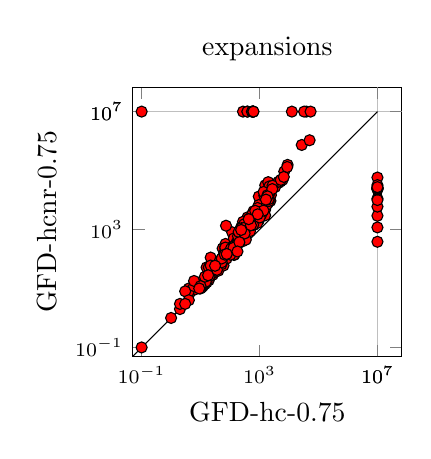
\begin{tikzpicture}
\begin{axis}[extra x tick style={grid=major}, extra x ticks=10000000, extra y tick style={grid=major}, extra y ticks=10000000, height=5cm, legend cell align=left, legend style={at={(1.3, 0.5)}}, title=expansions, width=5cm, xlabel=GFD-hc-0.75, xmin=0.05, xmode=log, ylabel=GFD-hcnr-0.75, ymin=0.05, ymode=log]
\addplot[color=red, mark=*, mark options={{draw=black}}, only marks] coordinates {
(226, 967) (6, 9) (981, 3311) (2144, 17941) (439, 1855) (942, 13116) (47, 66) (2121, 9781) (12, 12) (214, 686) (110, 283) (372, 890) (371, 930) (396, 958) (5143, 42522) (391, 2589) (58, 76) (11, 11) (125, 358) (169, 800) (43, 63) (275, 1834) (288, 1393) (937, 3229) (6046, 48299) (2695, 34370) (8954, 156081) (240, 1209) (95, 190) (19, 19) (1, 1) (173, 573) (4, 10) (1564, 31775) (106, 230) (175, 395) (46, 62) (14, 14) (70, 149) (37, 51) (2333, 9377) (296, 797) (22, 35) (27062, 739115) (123, 244) (38725, 10000000) (56, 228) (36, 41) (136, 290) (18, 25) (6890, 92912) (901, 2892) (227, 673) (137, 137) (1337, 6876) (607, 10000000) (622, 1783) (1458, 14012) (651, 2599) (103, 192) (16, 16) (275, 10000000) (1651, 7795) (32536, 10000000) (307, 954) (2437, 14770) (4389, 38253) (1805, 9221) (730, 2078) (10000000, 11219) (68, 248) (359, 929) (947, 2049) (27, 60) (70, 100) (891, 4609) (10000000, 2923) (48, 63) (26, 29) (10000000, 1180) (131, 318) (10000000, 57999) (40, 40) (164, 345) (118, 808) (2, 2) (34, 47) (24, 43) (3378, 27691) (639, 1422) (1469, 6939) (2176, 16918) (580, 10000000) (123, 212) (26, 33) (390, 10000000) (845, 1668) (302, 1070) (90, 150) (144, 407) (284, 1110) (306, 1402) (387, 10000000) (417, 1764) (13, 19) (73, 146) (92, 154) (391, 1046) (2036, 11460) (4401, 41680) (205, 694) (100, 202) (4, 6) (10, 10) (54, 95) (770, 3093) (604, 10000000) (53, 66) (552, 2794) (27, 38) (302, 699) (1971, 40492) (251, 850) (259, 1053) (941, 6750) (112, 314) (56, 73) (476, 878) (1538, 4638) (4, 8) (188, 381) (550, 10000000) (22, 112) (419, 1653) (245, 463) (142, 142) (6, 12) (602, 2919) (271, 760) (2155, 29010) (11, 17) (10000000, 24484) (1940, 7993) (101, 240) (60, 60) (499, 1732) (276, 542) (606, 10000000) (51, 66) (1741, 6855) (10000000, 5974) (10000000, 384) (474, 2375) (1548, 3031) (2754, 30702) (129, 385) (235, 1133) (737, 3522) (70, 324) (6, 18) (173, 421) (77, 104) (57, 114) (20, 26) (301, 1508) (13, 15) (607, 1430) (67, 139) (10000000, 10018) (623, 4157) (2, 3) (338, 1116) (16, 52) (1373, 18842) (134, 497) (260, 395) (0.100000, 10000000) (622, 10000000) (979, 3145) (133, 272) (5263, 48377) (12503, 10000000) (70, 160) (2060, 9235) (6652, 60966) (10000000, 25685) (103, 140) (80, 160) (10000000, 32097) (15, 17) (2025, 10591) (1165, 3337) (164, 351) (1844, 14576) (19, 52) (14, 25) (73, 1348) (170, 340) (10000000, 22877) (45, 89) (28, 55) (96, 236) (246, 1106) (164, 302) (335, 1194) (36, 43) (861, 5382) (3, 8) (119, 254) (342, 450) (2708, 23542) (8690, 132345) (1018, 2560) (53916, 10000000) (10, 12) (136, 233) (83, 195) (297, 735) (64, 163) (10000000, 24217) (442, 2329) (186, 594) (10000000, 26130) (1875, 13298) (0.100000, 0.100000) (49941, 1067776) (253, 755) (1652, 10340) (4, 4) (9, 10) (1362, 4383) (69, 244) (52, 77) (106, 219) (52, 104) (131, 240) (22, 60) (564, 3227) (3, 3) (10000000, 27397) (196, 828) (311, 735) (511, 1394) (31, 59) (207, 372) (238, 966) (715, 4320) (66, 141) (867, 3283) (429, 2248) (77, 148) (178, 180) (18, 28)
};
\addplot[color=black] coordinates {(0.050000, 0.050000) (10000000, 10000000)};
\end{axis}
\end{tikzpicture}
	\end{minipage}
	\hfill
	\begin{minipage}{0.2\textwidth}
		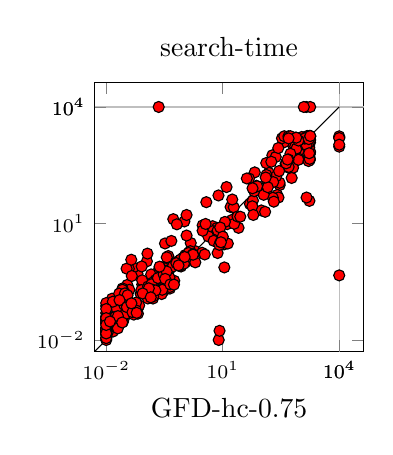
\begin{tikzpicture}
\begin{axis}[extra x tick style={grid=major}, extra x ticks=10000, extra y tick style={grid=major}, extra y ticks=10000, height=5cm, legend cell align=left, legend style={at={(1.3, 0.5)}}, title=search-time, width=5cm, xlabel=GFD-hc-0.75, xmin=0.005, xmode=log, ymin=0.005, ymode=log]
\addplot[color=red, mark=*, mark options={{draw=black}}, only marks] coordinates {
(0.028588, 0.035970) (0.698269, 1.030190) (0.034901, 0.262135) (98.691600, 21.673500) (0.012676, 0.017456) (1422.800045, 10000) (25.564400, 7.717710) (0.105115, 0.222073) (1.335820, 1.612330) (0.036071, 0.105629) (11.202300, 2.982330) (0.076990, 0.155101) (0.843372, 0.781518) (144.095000, 124.025000) (0.018737, 0.020747) (0.570090, 0.841492) (1733.526276, 605.803996) (0.066899, 0.069352) (0.063842, 0.506460) (1416.170875, 491.368920) (0.454279, 0.245628) (618.386006, 1200.902000) (1176.089915, 1605.396250) (118.259000, 61.971600) (0.152552, 0.316836) (0.962801, 1.322000) (1.118100, 1.017070) (0.244440, 0.749018) (0.010000, 0.032932) (0.010000, 0.016121) (0.039374, 0.195625) (388.243000, 1246.948000) (0.010000, 0.049424) (0.396773, 1.445910) (0.302142, 0.182898) (0.220770, 0.386856) (0.010000, 0.018436) (0.423347, 0.671825) (0.436588, 0.211109) (0.010000, 0.020001) (5.507420, 8.492880) (0.010000, 0.039269) (5.946540, 4.102760) (0.050820, 0.052995) (189.706000, 570.274000) (0.084698, 0.268282) (8.545920, 5.732110) (0.469501, 0.765802) (335.541000, 1564.624900) (0.450930, 0.818710) (7.133740, 7.685290) (0.318468, 0.704218) (50.208900, 31.798800) (0.326686, 3.059300) (416.354400, 345.446000) (5.594140, 6.334900) (1139.970000, 651.004000) (13.042300, 9.604810) (1746.234199, 432.524000) (0.049577, 0.738745) (59.958900, 38.902000) (1661.289171, 980.985170) (10000, 0.460674) (0.127264, 0.229988) (153.017000, 202.573000) (1714.700000, 457.336000) (757.336000, 1621.768800) (0.533816, 12.912700) (0.103409, 0.156985) (0.010000, 0.016005) (0.336299, 0.241045) (1.871030, 1.983460) (0.373961, 0.613401) (74.101300, 93.549400) (0.263021, 0.331453) (0.010000, 0.028483) (663.965000, 982.524200) (0.010000, 0.010000) (0.053153, 0.084408) (0.143701, 0.487279) (0.315772, 0.528561) (0.125928, 0.266322) (15.971500, 26.517700) (10000, 1627.377000) (0.904065, 1.232310) (1653.493405, 1492.140000) (10.286000, 3.358718) (1734.216734, 1796.834337) (0.030145, 0.057020) (475.666000, 278.382000) (0.084153, 0.343040) (7.384120, 1.734830) (0.010000, 0.074921) (66.795400, 206.862000) (0.232067, 0.677463) (1771.206562, 1776.525491) (293.137000, 97.591500) (0.017690, 0.029102) (0.159844, 0.116764) (131.815000, 359.863000) (1.029050, 11.276500) (1777.786578, 1731.373869) (1576.194000, 1674.393870) (0.065549, 0.047611) (0.010000, 0.013917) (0.010000, 0.036370) (1601.616220, 1300.257900) (1.081090, 1.534530) (0.018450, 0.065498) (3.038280, 8.932370) (0.027012, 0.029451) (1772.544357, 680.193979) (0.014849, 0.038325) (253.232000, 54.240800) (231.511000, 515.519147) (1658.562848, 870.148000) (131.346000, 64.949900) (0.035041, 0.067848) (0.014871, 0.016477) (0.475678, 3.550930) (10.809500, 2.896730) (10000, 1753.719500) (0.010866, 0.015410) (0.184775, 0.346383) (1685.361045, 1620.700000) (1.363950, 1.807730) (291.055000, 111.819000) (7.883260, 0.010000) (0.010000, 0.037374) (0.014167, 0.115752) (0.038213, 0.686321) (2.944550, 1.757220) (272.660000, 46.547300) (19.249400, 26.174800) (0.010000, 0.014208) (0.010000, 0.039580) (729.912000, 759.860000) (17.167000, 12.272200) (269.487506, 876.439600) (12.545600, 86.675500) (1.232960, 1.583710) (1081.618000, 1683.722300) (0.010000, 0.014132) (1766.634333, 1454.299136) (238.358000, 164.904000) (0.432221, 0.231120) (133.297000, 177.370000) (1663.683066, 1029.436750) (6.131140, 4.933490) (3.438020, 1.593020) (1758.205376, 1783.781586) (0.241276, 0.761414) (4.241070, 4.658860) (0.018404, 0.032512) (0.340572, 0.567627) (178.420000, 388.468952) (0.026297, 0.212369) (1724.742241, 645.736376) (0.070491, 0.077937) (0.267863, 0.152378) (804.670851, 1251.917400) (1762.888509, 721.047395) (0.010000, 0.017790) (0.033467, 0.687249) (0.163898, 0.307332) (1710.714415, 472.406000) (736.310000, 966.082000) (0.768340, 0.805476) (195.737000, 45.792900) (0.289497, 0.489038) (1.171650, 1.519770) (1.499469, 3.149330) (1764.762762, 1774.312790) (797.833000, 851.828000) (10000, 1583.554410) (0.617453, 0.880767) (0.080374, 0.192335) (8.277621, 0.017239) (0.564514, 0.334235) (1.661630, 1.133660) (0.019170, 0.039287) (0.025970, 0.196207) (0.051357, 0.045143) (648.176000, 272.150000) (0.021555, 0.156546) (1706.816900, 38.194500) (1687.463564, 904.648000) (0.742419, 1.086250) (1769.236499, 1218.177735) (1777.474492, 1380.888007) (0.017191, 0.039380) (10000, 951.470000) (113.268000, 54.767500) (0.361975, 1.344350) (0.819187, 1.177050) (948.512000, 455.875200) (0.045573, 0.444270) (0.010000, 0.020635) (1.463290, 1.934800) (0.058774, 0.091804) (497.959000, 285.837000) (0.010000, 0.089398) (1777.311833, 1747.171998) (19.678900, 9.818420) (0.161930, 0.133293) (0.120127, 0.239013) (0.058588, 0.057626) (891.031404, 436.559000) (0.117956, 0.117137) (1.174530, 4.896350) (1443.271400, 46.609200) (7.428120, 6.663120) (552.948000, 624.165201) (64.589600, 67.959200) (1660.644432, 882.358779) (1.323910, 1.743490) (1677.742200, 1722.741599) (0.030760, 0.046291) (0.146152, 0.271620) (1370.380000, 1027.360210) (0.258260, 0.432374) (0.010000, 0.026408) (1.425550, 1.400550) (1498.918146, 1791.039614) (1644.928015, 1190.920880) (0.010000, 0.030849) (0.342286, 0.258845) (1439.650000, 1050.638464) (0.028802, 0.081152) (0.019917, 0.019882) (3.781240, 35.365400) (1.969290, 0.996813) (283.281000, 224.346000) (0.010000, 0.018720) (0.010000, 0.014581) (0.010000, 0.037315) (1286.010000, 1541.540000) (0.014809, 0.096894) (1.722500, 1.619850) (0.111626, 1.059350) (1619.952000, 1749.966330) (0.214483, 0.394041) (0.277105, 0.196267) (1592.030000, 603.806000) (493.277000, 443.094000) (0.030347, 0.158542) (0.159614, 0.195324) (0.020044, 0.041174) (0.184487, 0.187838) (0.301257, 0.488516) (206.741000, 36.417300) (0.010000, 0.011416) (3.036980, 6.504920) (596.206000, 148.614000) (199.589000, 116.222000) (0.010000, 0.062724) (1789.482011, 10000) (1707.853347, 515.476248) (13.526000, 3.043170) (0.035383, 0.142023) (0.224661, 10000) (0.034147, 0.075056) (77.161700, 90.582500) (1.720740, 1.572360) (47.429400, 143.774000) (0.021989, 0.106302) (1623.614532, 405.088000) (383.890000, 1762.908200) (0.034113, 0.070111) (0.125204, 0.214028) (0.518536, 0.779330) (0.640766, 0.952026) (1227.620049, 10000) (431.008200, 353.447000) (0.047489, 0.051975) (144.822000, 85.855617) (123.469000, 19.974600) (1.172390, 16.541900) (467.231000, 442.250000) (0.010000, 0.011177) (0.010000, 0.014748) (57.722400, 27.684000) (11.375700, 10.975200) (3.619580, 9.717080) (0.425383, 0.404327) (41.795800, 144.178000) (8.615770, 7.887453) (1.001990, 0.921792) (7.770440, 52.692900) (1303.219013, 1556.323630) (0.360615, 0.580445) (5.839410, 3.578390) (17.591600, 41.409400) (0.010000, 0.036523) (0.328808, 0.374332) (1730.882848, 460.795000) (0.236435, 0.771949) (8.162680, 2.819640) (11.014700, 0.738677) (0.060770, 0.049957) (1.047520, 1.369580) (8.794420, 3.365036) (888.817047, 1367.304900) (0.082029, 0.782949) (0.086820, 0.157739) (128.033000, 152.502000) (0.658473, 9.510060) (1681.779983, 643.561000) (0.010000, 0.024396) (0.115375, 1.675830) (0.044538, 0.087778) (492.439000, 1759.505530) (24.114600, 15.114100) (552.977460, 1768.530000) (0.025835, 0.028197) (10.037100, 4.579630) (58.608700, 80.624300) (0.446390, 0.269813) (1646.521945, 1487.977000) (780.534925, 1620.694779) (0.012502, 0.029946) (10000, 1068.097000) (61.306800, 16.581000) (0.044197, 1.165820) (1795.541050, 1785.137790) (28.354100, 14.943300) (8.982500, 3.279597) (0.727492, 0.834750) (0.554831, 0.266699) (0.140079, 0.125292) (497.025000, 1552.814030)
};
\addplot[color=black] coordinates {(0.0050000, 0.0050000) (10000, 10000)};
\end{axis}
\end{tikzpicture}
	\end{minipage}

	\caption{Comparison of expansions and search time per task of $h^{C}$ with and 
	without the reuse of the heuristic for oversubscription IPC domains}
\end{figure}


\FloatBarrier
\newpage
\subsubsection*{Action Set Properties}

\begin{figure}[ht]
	\begin{tikzpicture}
\begin{axis}[extra x tick style={grid=major}, extra x ticks=100000000, 
	extra y tick style={grid=major}, extra y ticks=100000000, height=6cm, 
	legend cell align=left, legend style={at={(1.3, -0.5)}}, title=expansions, 
	width=6cm, xlabel=asp-hmax-GFD, xmin=100, xmode=log, ylabel=asp-hc-GFD, ymin=100, ymode=log]
\addplot[color=blue, mark=*, mark options={{draw=black}}, only marks] coordinates {
(14130, 4672) (100000000, 19516) (6949, 1387) (3003597, 14394) (51670929, 93760) (327036, 10492) (100000000, 39593) (119756, 8806) (21152030, 100000000) (4551, 606) (177854, 45225) (7770, 1227) (10157013, 72997) (87180, 3492) (481214, 5662) (47345, 1613) (802101, 17735) (10361851, 74595)
};
%\addlegendentry{blocked roads}
\addplot[color=cyan, mark=*, mark options={{draw=black}}, only marks] coordinates {
(11477521, 100000000) (127850, 11277) (369554, 8571) (122630, 3104) (454715, 5297) (190335, 5111) (33351, 1020) (433815, 5581) (42782, 2029)
};
%\addlegendentry{blocked roads 2T}
\addplot[color=red, mark=*, mark options={{draw=black}}, only marks] coordinates {
(2995530, 18623) (31395453, 100000000) (100843, 5361) (127212, 32109) (18512, 5374) (1083857, 6283) (336360, 27850) (10173, 1067) (28902543, 100000000) (50407796, 100000000) (473783, 87328) (97121, 4361) (5020, 1024) (556154, 11211) (24976, 3815) (23372256, 100000000)
};
%\addlegendentry{forced roads}
\addplot[color=orange, mark=*, mark options={{draw=black}}, only marks] coordinates {
(30461900, 100000000) (164075, 15012) (276396, 54970) (43112, 9472) (442653, 73187) (45990, 5368) (86968, 8492) (379662, 47842) (662286, 10711) (261961, 83116)
};
%\addlegendentry{forced roads 2T}
\addplot[color=yellow, mark=*, mark options={{draw=black}}, only marks] coordinates {
(2476390, 155698) (2182985, 76718) (171406, 25523) (3709462, 78224) (306141, 33941) (9214575, 100000000) (182936, 10924) (1813256, 212276) (578050, 62426)
};
%\addlegendentry{forced roads 5 2T}
\addplot[color=green, mark=*, mark options={{draw=black}}, only marks] coordinates {
(15380934, 100000000) (25911962, 100000000) (33104624, 100000000) (5499358, 100000000) (1308157, 86092) (5635233, 100000000) (22855461, 100000000) (2962444, 100000000) (6945248, 100000000)
};
%\addlegendentry{same truck 2T}
\addplot[color=darkgreen, mark=*, mark options={{draw=black}}, only marks] coordinates {
(9081, 176) (16558, 319) (2616728, 100000000) (6336, 462) (285248, 3635) (2108, 176) (39463, 1010) (104361, 234) (1653780, 21898) (44263267, 100000000)
};
%\addlegendentry{same truck with P0 2T}
\addplot[color=black] coordinates {(0.050000, 0.050000) (100000000, 100000000)};
\end{axis}
\end{tikzpicture}

	\begin{tikzpicture}
\begin{axis}[extra x tick style={grid=major}, extra x ticks=10000, 
	extra y tick style={grid=major}, extra y ticks=10000, height=6cm, 
	legend cell align=left, legend style={at={(0.9, -0.3)}}, title=search-time, 
	width=6cm, xlabel=asp-hmax-GFD, xmin=0.005, xmode=log, ylabel=asp-hc-GFD, ymin=0.005, ymode=log]
\addplot[color=blue, mark=*, mark options={{draw=black}}, only marks] coordinates {
(3.000890, 81.811600) (1.131580, 1.458470) (13.319200, 6.637240) (0.353865, 0.198306) (85.232500, 19.691200) (14.997400, 23.659700) (646.510000, 10000) (0.112922, 0.016453) (993.857000, 918.556000) (2.442110, 4.498780) (372.842000, 267.636000) (10000, 161.667000) (0.199281, 0.133952) (10.123400, 28.868500) (10000, 110.930000) (0.134073, 0.093680) (1.205280, 1.793270) (282.845000, 664.828000)
};
\addlegendentry{blocked roads}
\addplot[color=cyan, mark=*, mark options={{draw=black}}, only marks] coordinates {
(8.964480, 16.038800) (13.140700, 70.392600) (4.852950, 19.411200) (337.706000, 346.443000) (0.722817, 1.455130) (2.137660, 2.186500) (2.955610, 11.404700) (1.116110, 6.419080) (9.538120, 29.712400)
};
\addlegendentry{blocked roads 2T}
\addplot[color=red, mark=*, mark options={{draw=black}}, only marks] coordinates {
(0.122506, 0.063470) (628.818000, 10000) (0.425890, 4.595660) (15.600200, 12.727900) (702.433000, 10000) (0.554129, 0.597915) (11.175300, 174.963000) (2.408420, 20.600400) (0.229445, 0.075522) (7.084070, 20.647500) (1618.210000, 10000) (29.961400, 10.242900) (1006.310000, 10000) (2.468450, 12.658600) (78.106600, 19.433000) (1.395690, 2.286330)
};
\addlegendentry{forced roads}
\addplot[color=orange, mark=*, mark options={{draw=black}}, only marks] coordinates {
(3.004180, 4.469870) (7.808850, 59.706800) (874.548000, 10000) (10.247700, 156.019000) (1.365880, 17.711300) (1.064790, 3.498970) (1.638460, 9.276920) (20.753700, 126.607000) (8.748400, 99.734300) (9.865800, 145.352000)
};
\addlegendentry{forced roads 2T}
\addplot[color=yellow, mark=*, mark options={{draw=black}}, only marks] coordinates {
(4.704120, 31.647600) (84.431300, 1267.590000) (57.662700, 902.731000) (65.552300, 1565.490000) (7.074960, 16.753800) (15.269500, 99.041600) (1786.728120, 10000) (83.578600, 964.151000) (335.518000, 1006.810000) (8.221520, 46.874100)
};
\addlegendentry{forced roads 5 2T}
\addplot[color=green, mark=*, mark options={{draw=black}}, only marks] coordinates {
(172.493000, 10000) (50.368900, 3304.200000) (160.456000, 10000) (961.137000, 10000) (318.710000, 10000) (107.134000, 10000) (1037.090000, 10000) (579.746000, 10000) (701.169000, 10000)
};
\addlegendentry{same truck 2T}
\addplot[color=darkgreen, mark=*, mark options={{draw=black}}, only marks] coordinates {
(0.063412, 0.081935) (2.124110, 0.160501) (1.075250, 1.713790) (36.566500, 96.990600) (0.733713, 0.102953) (4.795050, 15.541000) (0.179801, 0.010000) (1256.840000, 10000) (0.156679, 0.277623) (78.002100, 10000)
};
\addlegendentry{same truck with P0 2T}
\addplot[color=black] coordinates {(0.0050000, 0.0050000) (10000, 10000)};
\end{axis}
\end{tikzpicture}

	\caption{Compare $h^C$ and $h^{max}$ with respect of different \emph{types} of action set properties. 
	one truck: forced and blocked roads, two trucks: blocked roads, two packages in the same truck}
\end{figure}

